\documentclass[AMA,STIX1COL]{WileyNJD-v2}

\articletype{Research Article}

\received{26 April 2016}
\revised{6 June 2016}
\accepted{6 June 2016}

\raggedbottom

%\usepackage{booktabs}

\let\procedure\relax
\let\endprocedure\relax

%\usepackage[ruled]{algorithm2e} % For algorithms

\usepackage[noline, noend, nofillcomment, linesnumbered]{algorithm2e}
%\usepackage[noline, noend, nofillcomment]{algorithm2e}
%\usepackage[noline, noend, nofillcomment, linesnumbered]{algorithm2e}
%    \setlength{\algomargin}{0em}

\usepackage{setspace}

\SetArgSty{textnormal}

% comments in the pseudocode
% note: on my system \texttt is broken with \small font size (too small)
\newcommand\Xcommentfont[1]{\selectfont\textnormal{#1}}
%\newcommand\Xcommentfont[1]{\fontsize{9pt}{0pt}\selectfont\texttt{#1}}
\SetCommentSty{Xcommentfont}
\SetNoFillComment

\let\oldnl\nl % Store \nl in \oldnl
\newcommand{\nonl}{\renewcommand{\nl}{\let\nl\oldnl}} % Remove line number for one line

\SetNlSty{textnormal}{}{}

\renewcommand{\algorithmcfname}{ALGORITHM}
%\SetAlFnt{\small}
%\SetAlCapFnt{\small}
%\SetAlCapNameFnt{\small}
%\SetAlCapHSkip{0pt}
%\IncMargin{-\parindent}

\usepackage[utf8]{inputenc}
\usepackage{amsmath, amssymb, amsthm, amsfonts}
\usepackage{accents}
\usepackage{mathtools}
\usepackage{graphicx}
\usepackage{enumitem}
\usepackage[justification=centering]{caption}
\usepackage{url}
\usepackage{vwcol}
\usepackage[section]{placeins}
\usepackage{proof-at-the-end}

\newcommand{\Xl}{\langle}
\newcommand{\Xr}{\rangle}
\newcommand{\Xm}{\langle\!\rangle}
\newcommand{\Xset}{\!\leftarrow\!}
\newcommand{\Xund}{\rule{.4em}{.4pt}}
\newcommand{\Xlb}{[\![}
\newcommand{\Xrb}{]\!]}
\newcommand{\Xmap}{\!\mapsto\!}
\newcommand{\XB}{\mathcal{B}}
\newcommand{\XD}{\mathcal{D}}
\newcommand{\XE}{\mathcal{E}}
\newcommand{\XF}{\mathcal{F}}
\newcommand{\XI}{\mathcal{I}}
\newcommand{\XPT}{\XP\!\XT}
\newcommand{\XIT}{\XI\!\XT}
\newcommand{\XIR}{\XI\!\XR}
\newcommand{\XL}{\mathcal{L}}
\newcommand{\XN}{\mathcal{N}}
\newcommand{\XM}{\mathcal{M}}
\newcommand{\XO}{\mathcal{O}}
\newcommand{\XP}{\mathcal{P}}
\newcommand{\XR}{\mathcal{R}}
\newcommand{\XS}{\mathcal{S}}
\newcommand{\XT}{\mathcal{T}}
\newcommand{\XX}{\mathcal{X}}
\newcommand{\YB}{\mathbb{B}}
\newcommand{\YC}{\mathbb{C}}
\newcommand{\YK}{\mathbb{K}}
\newcommand{\YF}{\mathbb{F}}
\newcommand{\YN}{\mathbb{N}}
\newcommand{\YT}{\mathbb{T}}
\newcommand{\YQ}{\mathbb{Q}}
\newcommand{\YP}{\mathbb{P}}
\newcommand{\YZ}{\mathbb{Z}}
\newcommand{\PT}{PT}
\newcommand{\PE}{P\!E}
\newcommand{\PR}{P\!R}
\newcommand{\IPT}{I\!PT}
\newcommand{\IRE}{I\!RE}

\newcommand{\Xstirling}[2]{\genfrac{\{}{\}}{0pt}{}{#1}{#2}}
\newcommand*{\Xbar}[1]{\overline{#1}}
\newcommand{\pnorm}[2]{\|{#1}\|^{pos}_{#2}}
\newcommand{\snorm}[2]{\|{#1}\|^{sub}_{#2}}

\DeclarePairedDelimiter\ceil{\lceil}{\rceil}
\DeclarePairedDelimiter\floor{\lfloor}{\rfloor}

\setlist{nosep}
%\setlength{\parskip}{0.5em}

\newenvironment{Xfig}
    {\par\medskip\noindent\minipage{\linewidth}\begin{center}}
    {\end{center}\endminipage\par\medskip}
\newenvironment{Xtab}
    {\par\medskip\noindent\minipage{\linewidth}\begin{center}}
    {\end{center}\endminipage\par\medskip}

\setlength{\parindent}{0pt}
\setlength{\belowcaptionskip}{-1em}


\begin{document}

\title{Efficient POSIX Submatch Extraction on NFA}

\author[1]{Angelo Borsotti}
\author[2]{Ulya Trofimovich}

\address[1]{\email{angelo.borsotti@mail.polimi.it}}
\address[2]{\email{skvadrik@gmail.com}}

\abstract[Summary]{
We give an algorithm for regular expression parsing and submatch extraction with POSIX longest-match semantics.
The algorithm is based on Okui-Suzuki disambiguation procedure with a few important extensions and improvements.
We study other NFA-based algorithms
and show that Kuklewicz algorithm is slower in practice,
and the backward matching algorithm by Cox is incorrect.
%
Our algorithm works in worst-case $O(n \, m^2 \, t)$ time and $O(m^2)$ space,
where $n$ is the length of input, $m$ is the size of the regular expression with counted repetition subexpressions ``unrolled'',
and $t$ is the number of capturing groups and subexpressions that contain them.
%
Benchmarks show that in practice our algorithm is about 5x slower than leftmost greedy matching
(which has no overhead on disambiguation).
%
We present a lazy variation that is much faster, but requires memory proportional to the size of input.
}

\keywords{Regular Expressions, Parsing, Submatch Extraction, Finite-State Automata, POSIX}

%\jnlcitation{\cname{
%\author{U. Trofimovich},
%(\cyear{2017}),
%\ctitle{Fast Submatch Extraction in Lexer Generators},
%\cjournal{Q.J.R. Meteorol. Soc.},
%\cvol{2017;00:1--6}.}

\maketitle

\section{Introduction}

In this paper we study NFA-based approaches to the problem of POSIX regular expression parsing and submatch extraction.
A number of algorithms have been proposed in recent years,
but not all of them were thoroughly studied and formalized,
and some support only a subset of POSIX regular expressions.
Our goal is to compare different approaches,
pick the most efficient one,
extend it on the full range of POSIX regular expressions
and provide a practical matching algorithm.
%
It should be noted that there exists a totally different approach to the problem based on Brzozowski derivatives.
We choose to focus on NFA-based approach for the following reasons:
first, we feel that both approaches deserve to be studied and formalized;
and second, in our experience derivative-based approach is slow in practice
(possibly due to an imperfect implementation, but we also discuss theoretical bounds below).
%
Both NFA and derivatives can be used to construct DFA with POSIX longest-match semantics [SL13] [Bor15] [Tro17].
The resulting DFA-based algorithms are very fast, because there is no run-time overhead on disambiguation.
However, DFA construction is not always viable due to its exponential worst-case complexity,
and if viable, it needs to be efficient.
Therefore we concentrate on NFA-based algorithms
that can be used directly for matching, or serve as a basis for DFA construction.
We give an overview of existing algorithms, including some that are incorrect but interesting.
%
\iffalse
The difficulty of POSIX longest-match semantics is caused by our inability to predict correct match results at the point where they diverge.
Consider regular expression \texttt{(a\{2\}|a\{3\}|a\{5\})*} and string \texttt{a...a}.
Submatch on the last iteration varies with the length of input:
it equals \texttt{aaaaa} for $5n$-character string,
\texttt{aa} for strings of length $5n - 3$ and $5n - 1$,
and \texttt{aaa} for strings of length $5n - 2$ and $5n + 1$ ($n \in \YN$).
Variation continues infinitely with a period of five characters.
The period is a property of regular expression;
in our example we can change it by choosing different counter values.
POSIX matching algorithms deal with this difficulty in different ways.
On one side we have generic, but inefficient approaches like exhaustive backtracking and dynamic programming.
On the other side we have algorithms based on deterministic automata [SL13] [Bor15] [Tro17]
that are very efficient at run-time, because all disambiguation is done in advance and built into DFA.
However, DFA construction is not always viable due to its exponential worst-case complexity,
and if viable, it needs to be efficient.
Therefore in this work we concentrate on practical NFA-based algorithms
that can be used directly for matching or serve as a basis for DFA construction.
We give an overview of existing algorithms, including some that are incorrect, but interesting.
\fi

\subparagraph{Laurikari, 2001 (incorrect).}

Laurikari algorithm is based on TNFA, which is an $\epsilon$-NFA with tagged transitions [Lau01].
Each submatch group is represented with a pair of \emph{tags} (opening and closing).
Disambiguation is based on minimizing the value of opening tags and maximizing tha value of closing tags, where
different tags have priority according to POSIX subexpression hierarchy.
Notably, Laurikari used the idea of topological order to avoid worst-case exponential time of $\epsilon$-closure construction.
His algorithm doesn't track history of iteration subexpressions and gives incorrect result in cases like \texttt{(a|aa)*} and string \texttt{aa}.
Reported computational complexity is $O(n \, m \, c \, t \, log(t))$, where
$n$ is input length,
$m$ is TNFA size,
$c$ is the time for comparing tag values
and $t$ is the number of tags.
Memory requirement is $O(m \, t)$.

\subparagraph{Kuklewicz, 2007.}

Kuklewicz fixed Laurikari algorithm by introducing \emph{orbit} tags for iteration subexpressions.
He gave only an informal description [Kuk07], but the algorithm was later formalized in [Tro17].
It works in the same way as Lauirikari algorithm,
except that comparison of orbit tags is based on their previous history, not just the most recent value.
The clever idea is to avoid recording full history
by compressing histories in a matrix of size $t \times m$, where $m$ is TNFA size and $t$ is the number of tags.
$t$-Th row of the matrix represents ordering of closure states with respect to $t$-th tag
(with possible ties --- different states may have the same order).
Matrix is updated at each step using continuations of tag histories.
The algorithm requires $O(m \, t)$ memory and $O(n \, m \, t \, (m + t \, log(m))$ time, where $n$ is the input length
($\epsilon$-closure takes $O(m^2 \, t)$ assuming worst-case optimal algorithm,
and matrix update takes $O(m \, log(m) \, t^2)$ because for $t$ tags we need to sort $m$ states with $O(t)$ comparison function).
%Kuklewicz disambiguation is combined with Laurikari determinization [Lau00] in [Tro17].

\subparagraph{Cox, 2009 (incorrect).}

Cox came up with the idea of backward POSIX matching,
which is based on the observation that it is easier to maximize submatch on the last iteration than on the first one,
because we do not need to track the full history of previous iterations.
The algorithm consumes input from right to left
and tracks two pairs of offsets for each submatch group:
the \emph{active} pair of the most recent offsets used in disambiguation,
and the \emph{final} pair of offsets on the backwards-first (i.e. the last) iteration.
The algorithm gives incorrect results under two conditions:
(1) ambiguous matches have equal offsets on some iteration,
and (2) disambiguation happens too late, when active offsets have already been updated and the difference between ambiguous matches is erased.
We found that such situations may occur for two reasons.
First, $\epsilon$-closure algorithm sometimes compares ambiguous paths \emph{after} their join point,
when both paths have a common suffix with tagged transitions.
This is the case with Cox prototype implementation [Cox09]; for example, it gives incorrect results for \texttt{(aa|a)*} and string \texttt{aaaaa}.
Most of such failures can be repaired by exploring states in topological order,
but topological order does not exist in the presence of $\epsilon$-loops.
The second reason is bounded repetition: ambiguous paths may not have an intermedite join point at all.
For example, in case of \texttt{(aaaa|aaa|a)\{3,4\}} and string \texttt{aaaaaaaaaa}
we have matches \texttt{(aaaa)(aaaa)(a)(a)} and \texttt{(aaaa)(aaa)(aaa)}
with different number of iterations.
Assuming that bounded repetion is modelled by chaining three non-optional sub-automata for \texttt{(aaaa|aaa|a)} and the optional fourth one,
by the time ambiguous paths meet both have active offsets \texttt{(0,4)}.
Despite the flaw, Cox algorithm is interesting: if somehow delayed comparison problem was fixed, it would work.
The algorithm requires $O(m \, t)$ memory and $O(n \, m^2 \, t)$ time
(assuming worst-case optimal closure algorithm),
where $n$ is the input length,
$m$ it the size of regular expression
and $t$ is the number of submatch groups plus enclosing subexpressions.

\subparagraph{Okui and Suzuki, 2013.}

Okui and Suzuki view disambiguation problem from the point of comparison of parse trees [OS13].
Ambiguous trees have the same sequence of leaf symbols, but their branching structure is different.
Each subtree corresponds to a subexpression.
The \emph{norm} of a subtree (the number of leaf symbols in it) equals to submatch length.
Longest match corresponds to a tree in which the norm of each subtree in leftmost in-order traversal is maximized.
The clever idea of Okui and Suzuki is to relate the norm of subtrees to their \emph{height} (distance from the root).
Namely, if we walk through the leaves of two ambiguous trees, tracking the height of each complete subtree,
then at some step heights will diverge:
subtree with a smaller norm will already be complete, but the one with a greater norm will not.
Height of subtrees is easy to track by attibuting it to parentheses and encoding in automaton transitions.
Okui and Suzuki use PAT --- $\epsilon$-free position automaton with transitions labelled by sequences of parentheses.
Disambiguation is based on comparing parentheses along ambiguous PAT paths.
Similar to Kuklewicz, Okui and Suzuki avoid recording full-length paths
by pre-comparing them at each step and storing comparison results in a pair of matrices indexed by PAT states.
The authors report complexity $O(n(m^2 + c))$, where
$n$ is the input length,
$m$ is the number of occurrences of the most frequent symbol in regular expression
and $c$ is the number of submatch groups and repetition operators.
However, this estimate leaves out the constuction of PAT and precomputation of precedence relation.
Memory requirement is $O(m^2)$.
Okui-Suzuki disambiguation is combined with Berry-Sethi construction in [Bor15] in construction of parsing DFA.

\subparagraph{Sulzmann and Lu, 2013.}

Sulzmann and Lu based their algorithm on Brzozowski derivatives [??]
(correctness proof is given by Ausaf, Dyckhoff and Urban [??]).
The algorithm unfolds a regular expression into a sequence of derivatives
(each derivative is obtained from the previous one by consuming the next input symbol),
and then folds it back into a parse tree
(the tree for the previous derivative is built from the tree for the next derivative by ``injecting'' the corresponding input symbol).
In practice, Sulzmann and Lu fuse backward and forward passes,
which allows to avoid potentially unbounded memory usage on keeping all intermediate derivatives.
The algorithm is unique in that it does not require explicit disambiguation: longest match is obtained by construction.
Time and space complexity is not entirely clear.
In [??] Sulzmann and Lu consider the size of the regular expression as a constant.
In [??] they give more precise estimates: $O(2^m \, t)$ space and $O(n \, log(2^m) \, 2^m \, t^2)$ time,
where $m$ is the size of the regular expression,
$n$ is the length of input
and $t$ the number of submatch groups (the authors do not differentiate between $m$ and $t$).
However, this estimate assumes worst-case $O(2^m)$ derivative size and on-the-fly DFA construction.
The authors also mention a better $O(m^2)$ theoretical bound for derivative size.
If we adopt it and exclude DFA consturuction, we get $O(m^2 \, t)$ memory requirement and $O(n \, m^2 \, t^2)$ time,
which seems reasonably close to NFA-based approaches.
\\

Undoubtedly, other approaches exist,
but many of them produce incorrect results or require memory proportional to the length of input
(e.g. Glibc implementation [??]).
%Of the two correct NFA-based approaches, Okui-Suzuki appears to be faster in practice.
%It should be noted that Okui-Suzuki and Kuklewicz approaches have much in common:
%both compare partial matches incrementally at each step,
%only Kuklewicz considers history of each tag separately.
%
Our contributions are the following:
\\[-0.5em]

\begin{itemize}[itemsep=0.5em]

    \item We extend Okui-Suzuki algorithm on the case of partially ordered parse trees.
        This results in significant reduction of the overhead on disambiguation
        for regular expressions with only a few submatch groups (a common case in practice).

    \item We extend Okui-Suzuki algorithm on the case of bounded repetition.

    \item We combine Okui-Suzuki algorithm with Laurikari TNFA.
        It allows us to omit the preprocessing step
        at the cost of $\epsilon$-closure construction,
        which may be preferable in cases when preprocessing time is included in match time.

    \item We introduce \emph{negative tags} that allow us to handle
        no-match situation in the same way as match.
        Negative tags provide a simple way to reset obsolete offsets from earlier iterations,
        in cases like \texttt{(a(b)?)*} and string \texttt{aba}.

    \item We consider $\epsilon$-closure construction as a shortest-path problem
        and show that path concatenation is right-distributive over path comparison
        for the subset of paths considered by closure algorithm.
        This justifies the use of well-known Goldberg-Radzik algorithm based on the idea of topological order,
        which has worst-case optimal quadratic complexity in the size of closure
        and guaranteed linear complexity if the closure has no $\epsilon$-loops.
        This is an improvement over naive exhaustive depth-first search with backtracking,
        and also an improvement over Laurikari algorithm as shown in [Tro17].

    \item We give a faster algorithm for updating precedence matrices.
        The straightforward algorithm described by Okui and Suzuki involves pairwise comparison of all states in closure
        and takes $O(m^2 \, t)$ time, assuming $m$ states and $O(t)$ comparison function.
        We show a pathological example \texttt{((a?)\{0,1000\})*} where $t \approx m$.
        Our algorithm takes $O(m^2)$ time.

    \item We show how to use our algorithm in order to build either parse trees or POSIX-style offsets.

    \item We present a simple \emph{lazy} variation of our algorithm
        that reduces the overhead on disambiguation
        at the cost of memory usage that grows with the length of input.
        The lazy algorithm is well-suited for small inputs.

    \item We provide a C++ implementation of different NFA-based algorithms
        and benchmark them against each other and against a ``baseline'' leftmost greedy implementation.
    \\[-0.5em]
\end{itemize}

The rest of this paper is arranged as follows.
In section \ref{section_main} we present the main idea and the skeleton of our algorithm.
In section \ref{section_formalization} we provide theoretical foundations for the rest of the paper.
After that, we go into specific details:
section \ref{section_closure} is concerned with $\epsilon$-closure construction,
section \ref{section_pathtree} discusses data structures used to represent TNFA paths,
section \ref{section_results} discusses possible output formats (parse trees or POSIX-style offsets),
section \ref{section_comparison} gives the core disambiguation algorithms,
section \ref{section_lazy} presents lazy variation of our algorithm,
and section \ref{section_tnfa} gives specific TNFA construction.
The remaining sections \ref{section_complexity}, \ref{section_benchmarks} and \ref{section_conclusion}
contain complexity analysis, benchmarks, conclusions and directions for future work.

\section{The main idea}\label{section_main}

Our algorithm is based on four cornerstone concepts:
regular expressions, parse trees, parenthesized expressions and tagged NFA.
%
First, we formalize the matching problem
by giving the usual interpretation of a regular expression as a set of parse trees.
%
Next, we define POSIX disambiguation semantics in terms of order on parse trees.
This definition reflects POSIX standard,
but it is too high-level to be used in a practical matching algorithm.
%
Therefore we go from parse trees to their linearized representation --- parenthesized expressions.
We define order on parenthesized expressions and show its equivalence to the order on parse trees.
The latter definition of order is more low-level and can be easily converted to an efficient comparison procedure.
%
Finally, we construct TNFA and map parenthesized expressions to its paths,
which allows us to compare ambiguous paths using the definition of order on parenthesized expressions.
%
Below are the four basic definitions and the skeleton of the algorithm.
In the following sections we formalize the relation between different representations and fill in all the details.

    \begin{definition}
    \emph{Regular expressions (RE)} over finite alphabet $\Sigma$, denoted $\XR_\Sigma$:
    \begin{enumerate}
        \item
          Empty RE $\epsilon$ and
          unit RE $\alpha$ (where $\alpha \in \Sigma$) are in $\XR_\Sigma$.
        \item If $e_1, e_2 \in \XR_\Sigma$, then
          union $e_1 | e_2$,
          product $e_1 e_2$,
          repetition $e_1^{n, m}$ (where $0 \leq n \leq m \leq \infty$), and
          submatch group $(e_1)$
          are in $\XR_\Sigma$.
    \end{enumerate}
    \end{definition}


    \begin{definition}
    \emph{Parse trees (PT)} over finite alphabet $\Sigma$, denoted $\XT_\Sigma$:
    \begin{enumerate}
        \item
          Nil tree ${\varnothing}^i$,
          empty tree ${\epsilon}^i$ and
          unit tree ${\alpha}^i$ (where $\alpha \in \Sigma$ and $i \in \YZ$)
          are in $\XT_\Sigma$.
        \item If $t_1, \dots, t_n \in \XT_\Sigma$ (where $n \geq 1$, and $i \in \YZ$), then
          ${T}^i(t_1, \dots, t_n)$
          is in $\XT_\Sigma$.
    \end{enumerate}
    \end{definition}


    \begin{definition}
    \emph{Parenthesized expressions (PE)} over finite alphabet $\Sigma$, denoted $\XP_\Sigma$:
    \begin{enumerate}
        \item
            Nil expression $\Xm$,
            empty expression $\epsilon$ and
            unit expression $\alpha$ (where $\alpha \in \Sigma$)
            are in $\XP_\Sigma$.
        \item If $e_1, e_2 \in \XP_\Sigma$, then
            $e_1 e_2$ and
            $\Xl e_1 \Xr$
            are in $\XP_\Sigma$.
    \end{enumerate}
    \end{definition}


    \begin{definition}
    \emph{Tagged Nondeterministic Finite Automaton (TNFA)}
    is a structure $(\Sigma, Q, T, \Delta, q_0, q_f)$, where:
    \begin{itemize}
        \item[] $\Sigma$ is a finite set of symbols (\emph{alphabet})
        \item[] $Q$ is a finite set of \emph{states}
        \item[] $T \subset \YN \times \YZ \times \YN \times \YN$ is a mapping of \emph{tags} to their submatch group, lower nested tag and upper nested tag
        \item[] $\Delta = \Delta^\Sigma \sqcup \Delta^\epsilon$ is the \emph{transition} relation,
            consisting of two parts:
        \begin{itemize}
            \item[] $\Delta^\Sigma \subseteq Q \times \Sigma \times \{\epsilon\} \times Q$ (transitions on symbols)
            \item[] $\Delta^\epsilon \subseteq Q \times \YN \times \big( \YZ \cup \{\epsilon\} \big) \times Q$
                ($\epsilon$-transitions, where $\forall (q, n, \Xund, \Xund), (q, m, \Xund, \Xund) \in \Delta^\epsilon: n \neq m$)
        \end{itemize}
        \item[] $q_0 \in Q$ is the \emph{initial} state
        \item[] $q_f \in Q$ is the \emph{final} state
    \end{itemize}
    \end{definition}

As the reader might notice, our definitions are subtly different from the usual ones in literature.
Regular expressions are extended with submatch operator
and generalized repetition (note that it is not just syntactic sugar: in POSIX \texttt{(a)(a)} is semantically different from \texttt{(a)\{2\}},
and \texttt{(a)} in not the same as \texttt{a}).
Parse trees have a special \emph{nil-tree} constructor
and an upper index, which allows us to distinguish between submatch and non-submatch subtrees.
Mirroring parse trees, parenthesized expressions also have a special \emph{nil-parenthesis}.
TNFA is in essence a nondeterministic finite-state transducer
in which some of the $\epsilon$-transitions are marked with \emph{tags} ---
integer numbers that denote opening and closing parentheses of submatch groups.
For $i$-th group, opening tag is $2i - 1$ and closing tag is $2i$ (where $i \in \YN$).
Tags can be negative, which represents the absence of match and corresponds to nil-parenthesis $\Xm$ and nil-tree $\varnothing$.
Additionally, all $\epsilon$-transitions are marked with \emph{priority}
which allows us to impose specific order of TNFA traversal
(all $\epsilon$-transitions from the same state have different priority).
\\

\begin{algorithm}[H] \DontPrintSemicolon \SetKwProg{Fn}{}{}{} \SetAlgoInsideSkip{medskip}\label{alg_match}
\setstretch{0.8}
\Fn {$\underline{match \big( N \!\!=\! (\Sigma, Q, T, \Delta, q_0, q_f), \; \alpha_1 \!\hdots\! \alpha_n \big)} \smallskip$} {

    $B, D : \text{uninitialized matrices in } \YZ^{|Q| \times |Q|}, \; U: \text{path context}$ \;
    $r_0 = initial \Xund result(T)$ \;
    $u_0 = empty \Xund path(\,)$ \;
    $X = \big\{ (q_0, \varnothing, u_0, r_0) \big\}, \; i = 1$ \;

    \BlankLine
    \While {$i \leq n \wedge X \neq \emptyset$} {
        $X = closure(N, X, U, B, D)$ \;
        $X = update \Xund result(T, X, U, i, \alpha_i)$ \;
        $(B, D) = update \Xund ptables(N, X, U, B, D)$ \;
        $X = \big\{ (q, o, u_0, r) \mid (o, \Xund, \Xund, r) \in X \wedge (o, \alpha_i, \epsilon, q) \in \Delta^\Sigma \big\}$ \;
        $i = i + 1$ \;
    }

    \BlankLine
    $X = closure(N, X, U, B, D)$ \;
    \If {$(q_f, \Xund, u, r) \in X$} {
        \Return $f\!inal \Xund result (T, U, u, r, n)$
    } \lElse {
        \Return $\varnothing$
    }

    \BlankLine
}
%\caption{Skeleton of the matching algorithm.}
\caption{TNFA simulation on a string.}
\end{algorithm}
\medskip

The algorithm takes automaton $N$ and string $\alpha_1 \!\hdots\! \alpha_n$ as input,
and outputs match result is some form: it can be a parse tree or a POSIX array of offsets,
but for now we leave it unspecified and hide behind functions
$initial \Xund result ()$, $update \Xund result ()$ and $f\!inal \Xund result ()$.
The algorithm works by consuming input symbols,
tracking a set of active \emph{configurations}
and updating \emph{precedence tables} $B$ and $D$.
Configuration is a tuple $(q, o, u, r)$.
The first component $q$ is a TNFA state that is unique for each configuration in the current set.
Components $o$ and $u$ keep information about the path by which $q$ was reached:
$o$ is the \emph{origin} state used as index in precedence tables,
and $u$ is a path fragment constructed by $closure()$.
Specific representation of path fragments is hidden behind path context $U$ and function stub $empty \Xund path ()$.
Finally, $r$-component is a partial match result associated with state $q$.
Most of the real work happens inside of $closure()$ and $update \Xund ptables ()$, both of which remain undefined for now.
The $closure()$ function builds $\epsilon$-closure of the current configuration set:
it explores all states reachable by $\epsilon$-transitions from the $q$-components
and tracks the best path to each reachable state.
The $update \Xund ptables ()$ function
performs pairwise comparison of all configurations in the new set,
recording results in $B$ and $D$ matrices.
On the next step $q$-components become $o$-components.
If paths originating from current configurations meet on some future step,
$closure ()$ will use origin states to lookup comparison results in $B$ and $D$ matrices.
If the paths do not meet, then comparison performed by $update \Xund ptables ()$ is redundant ---
unfortunately we do not know in advance which configurations will spawn ambiguous paths.
\\

%\vfill\null

\section{Formalization}\label{section_formalization}

In this section we establish the relation between all intermediate representations.
For readability all proofs are moved to appendix.
%
First of all, we rewrite REs in a form that makes submatch information explicit:
to each subexpression we assign an \emph{implicit} and \emph{explicit} submatch index, where
explicit indices enumerate submatch groups (for all other subexpressions they are zero),
and implicit indices enumerate submatch groups and subexpressions that are not submatch groups,
but contain nested or sibling groups and need to be considered by disambiguation.
This form reflects POSIX standard, which states that
submatch extraction applies only to parenthesized subexpressions,
but the longest-match rule applies to all subexpressions regardless of parentheses.

    \begin{definition}
    \emph{Indexed regular expressions (IRE)} over finite alphabet $\Sigma$, denoted $\XIR_\Sigma$:
    \begin{enumerate}
        \item
          Empty IRE $(i, j, \epsilon)$ and
          unit IRE $(i, j, \alpha)$, where $\alpha \in \Sigma$ and $i, j \in \YZ$,
          are in $\XIR_\Sigma$.

        \item If $r_1, r_2 \in \XIR_\Sigma$ and $i, j \in \YZ$, then
          union $(i, j, r_1 \mid r_2)$,
          product $(i, j, r_1 \cdot r_2)$ and
          repetition $(i, j, r_1^{n, m})$, where $0 \leq n \leq m \leq \infty$,
          are in $\XIR_\Sigma$.
    \end{enumerate}
    \end{definition}

Function $\IRE$ transforms RE into IRE.
It is defined via a composition of two functions,
$mark()$ that transforms RE into IRE with submatch indices in the boolean range $\{0, 1\}$,
and $enum()$ that substitutes boolean indices with consecutive numbers.
An example of constructing an IRE from a RE is given on figure \ref{fig_mark_enum}.
%
    \begin{align*}
    &\begin{aligned}
        mark &: \XR_\Sigma \longrightarrow \XIR_\Sigma \\
        mark &(x) \mid_{x \in \{\epsilon, \alpha\}} = (0, 0, x) \\[-0.2em]
        %
        mark &(e_1 \circ e_2) \mid_{\circ \in \{|,\cdot\}} = (i, 0,
            (i, j_1, r_1) \circ
            (i, j_2, r_2)
            ) \\[-0.2em]
            &\text{where }            (i_1, j_1, r_1) = mark(e_1) \\[-0.2em]
            &\space{\hphantom{where }}(i_2, j_2, r_2) = mark(e_2) \\[-0.2em]
            &\space{\hphantom{where }}i = i_1 \vee i_2 \\[-0.2em]
        %
        mark &(e^{n, m}) \mid_{e = (e_1)} = (1, 0, (1, 1, r)) \\[-0.2em]
            &\text{where } (\Xund, \Xund, r) = mark(e_1) \\[-0.2em]
        %
        mark &(e^{n, m}) \mid_{e \neq (e_1)} = (i, 0, (i, j, r)) \\[-0.2em]
            &\text{where } (i, j, r) = mark(e) \\[-0.2em]
        %
        mark &((e)) = mark((e)^{1, 1})
    \end{aligned}
    %
    &&\begin{aligned}
        enum &: \YZ \times \YZ \times \XIR_\Sigma \longrightarrow \YZ \times \YZ \times \XIR_\Sigma \\
        enum &(\bar{i}, \bar{j}, (i, j, x)) \mid_{x \in \{\epsilon, \alpha\}}
            = (\bar{i} + i, \bar{j} + j, (\bar{i} \times i, \bar{j} \times j, x))
        \\[-0.2em]
        enum &(\bar{i}, \bar{j}, (i, j, r_1 \circ r_2)) \mid_{\circ \in \{|,\cdot\}}
            = (i_2, j_2, (\bar{i} \times i, \bar{j} \times j, \bar{r}_1 \circ \bar{r}_2)) \\[-0.2em]
            &\text{where }            (i_1, j_1, \bar{r}_1) = enum(\bar{i} + i, \bar{j} + j, r_1) \\[-0.2em]
            &\space{\hphantom{where }}(i_2, j_2, \bar{r}_2) = enum(i_1, j_1, r_2)
        \\[-0.2em]
        enum &(\bar{i}, \bar{j}, (i, j, r^{n,m})) = (i_1, j_1, (\bar{i} \times i, \bar{j} \times j, \bar{r}^{n,m})) \\[-0.2em]
            &\text{where }
                (i_1, j_1, \bar{r}) = enum(\bar{i} + i, \bar{j} + j, r)
        \\[-0.2em]
        \\[-0.2em]
        \IRE &: \XR_\Sigma \rightarrow \XIR_\Sigma \\[-0.2em]
        \IRE&(e) = r \\[-0.2em]
            &\text{where }(\Xund, \Xund, r) = enum(1, 1, mark(e))
        \\[-0.2em]
    \end{aligned}
    \end{align*}

The relation between regular expressions and parse trees is given by the operator $\PT$.
Each IRE denotes a set of PTs.
%
We write $str(t)$ to denote the string formed by concatenation of all alphabet symbols in the left-to-right traversal of $t$,
and $\PT(r, w)$ denotes the set $\big\{ t \in \PT(\IRE(r)) \mid str(t) = w \big\}$ of all PTs for a RE $r$ and a string $w$.
%
    \begin{align*}
        \PT &: \XIR_\Sigma \rightarrow 2^{\XT_\Sigma}
        \\
        \PT\big((i, \Xund, \epsilon)\big) &= \{ {\epsilon}^{i} \}
        \\[-0.2em]
        \PT\big((i, \Xund, \alpha)\big) &= \{ {\alpha}^{i} \}
        \\[-0.2em]
        \PT\big((i, \Xund, (i_1, j_1, r_1) \mid (i_2, j_2, r_2))\big) &=
            \big\{ {T}^{i}(t, \varnothing^{i_2}) \mid t \in \PT\big((i_1, j_1, r_1)\big) \big\} \cup
            \big\{ {T}^{i}(\varnothing^{i_1}, t) \mid t \in \PT\big((i_2, j_2, r_2)\big) \big\}
        \\[-0.2em]
        \PT\big((i, \Xund, (i_1, j_1, r_1) \cdot (i_2, j_2, r_2))\big) &=
            \big\{ {T}^{i}(t_1, t_2) \mid
                t_1 \in \PT\big((i_1, j_1, r_1)\big),
                t_2 \in \PT\big((i_2, j_2, r_2)\big)
            \big\} \\[-0.2em]
        \PT\big((i, \Xund, (i_1, j_1, r_1)^{n, m})\big) &=
            \begin{cases}
                \big\{ {T}^{i}(t_1, \dots, t_m) \mid t_k \in \PT\big((i_1, j_1, r_1)\big) \;
                    \forall k = \overline{1, m} \big\} \cup \{ {T}^{i}(\varnothing^{i_1}) \} &\text{if } n = 0 \\[-0.2em]
                \big\{ {T}^{i}(t_n, \dots, t_m) \mid t_k \in \PT\big((i_1, j_1, r_1)\big) \;
                    \forall k = \overline{n, m} \big\} &\text{if } n > 0
            \end{cases}
    \end{align*}
    \medskip

    \begin{definition}\label{ambiguity_of_parse_trees}
    \emph{Ambiguity of parse trees.}
    PTs $s$ and $t$ are \emph{ambiguous} iff $s \neq t$ and $s, t \in PT(r, w)$ for some RE $r$ and string $w$.
    \end{definition}

Following \ref{OS13}, we assign \emph{positions} to the nodes of RE and PT.
The root position is $\Lambda$, and position of the $i$-th subtree of a tree with position $p$ is $p.i$
(we shorten $\|t\|_\Lambda$ as $\|t\|$).
The \emph{length} of position $p$, denoted $|p|$, is defined as $0$ for $\Lambda$ and $|p| + 1$ for $p.i$.
%The set of all positions is denoted $\XP$.
The subtree of a tree $t$ at position $p$ is denoted $t|_p$.
Position $p$ is a \emph{prefix} of position $q$ iff $q = p.p'$ for some $p'$,
and a \emph{proper prefix} if additionaly $p \neq q$.
Position $p$ is a \emph{sibling} of position $q$ iff $q = q'.i, p = q'.j$ for some $q'$ and $i,j \in \YN$.
Positions are ordered lexicographically.
The set of all positions of a tree $t$ is denoted $Pos(t)$.
Additionally, we define a set of \emph{submatch positions} as
$Sub(t) = \big\{ p \mid \exists t|_p = s^i : i \neq 0 \big\}$ ---
a subset of $Pos(t)$ that contains positions of subtrees with nonzero implicit submatch index.
Intuitively, this is the set of positions important from disambiguation perspective:
in the case of ambiguity we do not need to consider the full trees,
just the relevant parts of them.
%
PTs have two definitions of norm, one for $Pos$ and one for $Sub$,
which we call \emph{p-norm} and \emph{s-norm} respectively:

\begin{figure}\label{fig_mark_enum}
\includegraphics[width=\linewidth]{img/mark_enum.pdf}
\vspace{-2em}
\caption{
IRE for RE $(\epsilon|a^{0,\infty})(a|\epsilon)^{0,3}$
and examples of PTs for string $a$.
S-norm is marked with $\#$.
}
\end{figure}

%\FloatBarrier

    \begin{definition}\label{tnorm_of_PTs}
    The \emph{p-norm} and \emph{s-norm} of a PT $t$ at position $p$ are:
    \begin{align*}
        \pnorm{t}{p} =
            \begin{cases}
                -1          &\text{if } p \in Pos(t) \text{ and } t|_p = \varnothing^i  \\[-0.2em]
                |str(t|_p)| &\text{if } p \in Pos(t) \text{ and } t|_p \neq \varnothing^i \\[-0.2em]
                \infty      &\text{if } p \not\in Pos(t)
            \end{cases}
    \quad\quad\quad
        \snorm{t}{p} =
            \begin{cases}
                -1          &\text{if } p \in Sub(t) \text{ and } t|_p = \varnothing^i  \\[-0.2em]
                |str(t|_p)| &\text{if } p \in Sub(t) \text{ and } t|_p \neq \varnothing^i \\[-0.2em]
                \infty      &\text{if } p \not\in Sub(t)
            \end{cases}
    \end{align*}
    \end{definition}

Generally the norm of a subtree means the number of alphabet symbols in its leaves, with two exceptions.
First, for nil subtrees the norm is $-1$: intuitively, they have the lowest ``ranking'' among all possible subtrees.
Second, for inexistent subtrees (those with positions not in $Pos(t)$) the norm is infinite.
This may seem counterintuitive at first, but it makes sense in the presense of REs with empty repetition.
According to the POSIX, optional empty repetitions are not allowed, and our definition reflects this:
if a tree $s$ has a subtree $s|_p$ corresponding to an empty repetition,
and another tree $t$ has no subtree at position $p$,
then the infinite norm $\|t\|_p$ ``outranks'' $\|s\|_p$.
We define two orders on PTs:

    \begin{definition}[P-order on PTs]
    \label{total_order_on_PTs}
    Given parse trees $t, s \in PT(r, w)$, we say that $t <_p s$ w.r.t. \emph{desision position} $p$
    iff $\pnorm{t}{p} > \pnorm{s}{p}$ and $\pnorm{t}{q} = \pnorm{s}{q} \; \forall q < p$.
    We say that $t < s$ iff $t <_p s$ for some $p$.
    \end{definition}

    \begin{definition}[S-order on PTs]
    \label{partial_order_on_PTs}
    Given parse trees $t, s \in PT(r, w)$, we say that $t \prec_p s$ w.r.t. \emph{desision position} $p$ % $p \in Sub(t) \cup Sub(s)$
    iff $\snorm{t}{p} > \snorm{s}{p}$ and $\snorm{t}{q} = \snorm{s}{q} \; \forall q < p$.
    We say that $t \prec s$ iff $t \prec_p s$ for some $p$.
    \end{definition}

    \begin{definition}\label{incomparable_PTs}
    PTs $t$ and $s$ are \emph{incomparable}, denoted $t \sim s$,
    iff neither $t \prec s$, nor $s \prec t$.
    \end{definition}

\begin{theoremEnd}[restate, no link to proof, no link to theorem, category=theorem_porder_on_PTs]{theorem}
    \label{theorem_porder_on_PTs}
    P-order $<$ is a strict total order on $PT(e, w)$ for any RE $r$ and string $w$.
\end{theoremEnd}
\begin{proofEnd}
    We need to show that $<$ is transitive and trichotomous.

    \begin{itemize}[itemsep=0.5em]
        \item[(1)]
            Transitivity: we need to show that $\forall t, s, u \in PT(e,w): (t < s \wedge s < u) \implies t < u$.
            \\[0.5em]
            Let $t <_p s$ and $s <_q u$ for some positions $p$, $q$, and let $r = min (p, q)$.
            \\[0.5em]
            First, we show that $\pnorm{t}{r} > \pnorm{u}{r}$.
            If $p \leq q$, we have $\pnorm{t}{p} > \pnorm{s}{p}$ (implied by $t <_p s$)
            and $\pnorm{s}{p} \geq \pnorm{u}{p}$ (implied by $s <_q u \wedge p \leq q$),
            therefore $\pnorm{t}{p} > \pnorm{u}{p}$.
            Otherwise $p > q$, we have $\pnorm{t}{q} > \pnorm{u}{q}$ (implied by $s <_q u$)
            and $\pnorm{t}{q} = \pnorm{s}{q}$ (implied by $t <_p s \wedge q < p$),
            therefore $\pnorm{t}{q} > \pnorm{u}{q}$.
            \\[0.5em]
            Second, we show that $\forall r' < r : \pnorm{t}{r'} = \pnorm{u}{r'}$.
            We have $\pnorm{t}{r'} = \pnorm{s}{r'}$ (implied by $t <_p s \wedge r' < p$)
            and $\pnorm{s}{r'} = \pnorm{u}{r'}$ (implied by $s <_q u \wedge r' < q$),
            therefore $\pnorm{t}{r'} = \pnorm{u}{r'}$.

        \item[(2)]
            Trichotomy: we need to show that $\forall t, s \in PT(e,w)$
            exactly one of $t < s$, $s < t$ or $t = s$ holds.
            Consider the set of positions where norms of $t$ and $s$ disagree
            $P = \{p \in Pos(t) \cup Pos(s) : \pnorm{t}{p} \neq \pnorm{s}{p}\}$.

            \begin{itemize}[itemsep=0.5em]
                \item[(2.1)] First case: $P \neq \emptyset$.
                    We show that in this case exactly one of $t < s$ or $s < t$ is true
                    ($t \neq s$ is obvious).
                    \\[0.5em]
                    First, we show that at least one of $t < s$ or $s < t$ is true.
                    %
                    Let $p = min(P)$; it is well-defined since $P$ is non-empty, finite and lexicographically ordered.
                    %
                    For all $q < p$ we have $\pnorm{t}{q} = \pnorm{s}{q}$ (by definition of $p$
                    and because $\pnorm{t}{q} = \infty = \pnorm{s}{q}$ if $q \not\in Pos(t) \cup Pos(s)$).
                    %
                    Since $\pnorm{t}{p} \neq \pnorm{s}{p}$, we have either $t <_p s$ or $t <_p s$.
                    \\[0.5em]
                    Second, we show that at most one of $t < s$ or $s < t$ is true,
                    i.e. $<$ is asymmetric: $\forall t, s \in PT(e,w) : t < s \implies s \not< t$.
                    %
                    Suppose, on the contrary, that $t <_p s$ and $s <_q t$ for some $p$, $q$.
                    Without loss of generality let $p \leq q$.
                    On one hand $t <_p s$ implies $\pnorm{t}{p} > \pnorm{s}{p}$.
                    But on the other hand $s <_q t \wedge p \leq q$ implies $\pnorm{t}{p} \leq \pnorm{s}{p}$.
                    Contradiction.

                \item[(2.2)] Second case: $P = \emptyset$.
                    We show that in this case $t = s$.
                    \\[0.5em]
                    We have $Pos(t) = Pos(s)$ --- otherwise there is a position with norm $\infty$ in only one of the trees.
                    Therefore $t$ and $s$ have identical node structure.
                    %
                    By lemma \ref{lemma_positions} any position in $t$ and $s$ corresponds to the same position in $\IRE(e)$.
                    %
                    Since any position in $\IRE(e)$ coresponds to a unique explicit submatch index,
                    it must be that submatch indices of all nodes in $t$ and $s$ coincide.
                    %
                    Consider some position $p \in Pos(t)$.
                    If $p$ corresponds to an inner node, then both $t|_p$ and $s|_p$ are of the form $T^i(\hdots)$.
                    Otherwise, $p$ corresponds to a leaf node, which can be either $\varnothing$ or $\epsilon$ or $\alpha$.
                    Since all three have different norms ($-1$, $0$ and $1$ respectively),
                    and since $\pnorm{t}{p} = \pnorm{s}{p}$, it must be that $t|_p$ and $s|_p$ are identical.
            \end{itemize}
    \end{itemize}
\end{proofEnd}
\vspace{-0.5em}

\begin{theoremEnd}[restate, no link to proof, no link to theorem, category=theorem_sorder_on_PTs]{theorem}
    \label{theorem_sorder_on_PTs}
    S-order $\prec$ is a strict weak order on $PT(e, w)$ for any RE $r$ and string $w$.
\end{theoremEnd}
\begin{proofEnd}
    We need to show that $\prec$ is asymmetric and transitive, and incomparability relation $\sim$ is transitive.

    \begin{itemize}[itemsep=0.5em]
        \item[(1)]
            Asymmetry: we need to show that $\forall t, s \in PT(e,w): t \prec s \implies s \not\prec t$.
            \\[0.5em]
            Suppose, on the contrary, that $t \prec_p s$ and $s \prec_q t$ for some $p$, $q$.
            Without loss of generality let $p \leq q$.
            On one hand $t \prec_p s$ implies $\snorm{t}{p} > \snorm{s}{p}$.
            But on the other hand $s \prec_q t \wedge p \leq q$ implies $\snorm{t}{p} \leq \snorm{s}{p}$.
            Contradiction.

        \item[(2)]
            Transitivity: we need to show that $\forall t, s, u \in PT(e,w): (t \prec s \wedge s \prec u) \implies t \prec u$.
            \\[0.5em]
            Let $t \prec_p s$ and $s \prec_q u$ for some positions $p$, $q$, and let $r = min (p, q)$.
            \\[0.5em]
            First, we show that $\snorm{t}{r} > \snorm{u}{r}$.
            If $p \leq q$, we have $\snorm{t}{p} > \snorm{s}{p}$ (implied by $t \prec_p s$)
            and $\snorm{s}{p} \geq \snorm{u}{p}$ (implied by $s \prec_q u \wedge p \leq q$),
            therefore $\snorm{t}{p} > \snorm{u}{p}$.
            Otherwise $p > q$, we have $\snorm{t}{q} > \snorm{u}{q}$ (implied by $s \prec_q u$)
            and $\snorm{t}{q} = \snorm{s}{q}$ (implied by $t \prec_p s \wedge q < p$),
            therefore $\snorm{t}{q} > \snorm{u}{q}$.
            \\[0.5em]
            Second, we show that $\forall r' < r : \snorm{t}{r'} = \snorm{u}{r'}$.
            We have $\snorm{t}{r'} = \snorm{s}{r'}$ (implied by $t \prec_p s \wedge r' < p$)
            and $\snorm{s}{r'} = \snorm{u}{r'}$ (implied by $s \prec_q u \wedge r' < q$),
            therefore $\snorm{t}{r'} = \snorm{u}{r'}$.

        \item[(3)]
            Transitivity of incomparability: we need to show that $\forall t, s \in PT(e,w): (t \sim s \wedge s \sim u) \implies t \sim u$.
            \\[0.5em]
            By forward implication of lemma \ref{lemma_incomparability_equivdef}
            $t \sim s \Rightarrow \forall p : \snorm{t}{p} = \snorm{s}{p}$ and
            $s \sim u \Rightarrow \forall p : \snorm{s}{p} = \snorm{u}{p}$, therefore
            $(t \sim s \wedge s \sim u) \Rightarrow \forall p : \snorm{t}{p} = \snorm{u}{p} \Rightarrow t \sim u$
            by backward implication of lemma \ref{lemma_incomparability_equivdef}.
    \end{itemize}
\end{proofEnd}

The following theorem \ref{theorem_order_compat} establishes an important relation between P-order and S-order.
P-order is total, and there is a unique $<$-minimal tree $t_{min}$.
S-order is partial, it partitions all trees into equivalence classes
and there is a whole class of $\prec$-minimal trees $T_{min}$
(such trees coincide in submatch positions, but differ in some non-submatch positions).
Theorem \ref{theorem_order_compat} shows that $t_{min} \in T_{min}$.
This means that P-order and S-order ``agree'' on the notion of minimal tree:
we can continuously narrow down $T_{min}$ until we are left with $t_{min}$.
In practice, this means that adding more parentheses in RE does not drastically change submatch results.
%
Note that this doesn't mean that P-order is an extension of S-order:
the two orders may disagree.
For example, consider trees $t$ and $u$ on figure \ref{fig_mark_enum}:
on one hand $t \prec_{2.2} u$, because $\snorm{t}{2.2} = \infty > 0 = \snorm{u}{2.2}$ and s-norms at all preceding submatch positions agree;
on the other hand $u <_{1.1} t$, because $\pnorm{t}{1.1} = -1 < 0 = \pnorm{u}{1.1}$
and p-norms at all preceding positions agree.

\begin{theoremEnd}[restate, no link to proof, no link to theorem, category=theorem_order_compat]{theorem}
    \label{theorem_order_compat}
    For a RE $e$ and string $w$,
    let $t_{min}$ be the $<$-minimal tree in $\PT(e,w)$
    and let $T_{min}$ be the class of the $\prec$-minimal trees in $\PT(e,w)$.
    Then $t_{min} \in T_{min}$.
\end{theoremEnd}
\begin{proofEnd}
    Consider any $t \in T_{min}$.
    From $t$ we can construct another tree $t'$ in the following way.
    Consider all positions $p \in Sub(t)$ which are not proper prefixes of another position in $Sub(t)$.
    For each such position, $t|_p$ is itself a PT for some sub-IRE $r'$ and substring $w'$: $t|_p \in \PT(r', w')$.
    Let $t'_{min}$ be the $<$-minimal tree in $\PT(r', w')$ and substitute $t|_p$ with $t'_{min}$.
    Let $t'$ be the tree resulting from all such substitutions
    (note that they are independent of the order in which we consider positions $p$).
    Since substitutions preserve s-norm at submatch positions, we have $t' \in T_{min}$.
    We will show that $t' = t_{min}$.
    \\[0.5em]
    Suppose, on the contrary, that $t' \neq t_{min}$.
    %
    Then $t_{min} <_p t'$ for some decision position $p$.
    %
    It must be that $p \not\in Sub(t') \cup Sub(t_{min})$, because
    otherwise $\snorm{t_{min}}{p} = \pnorm{t_{min}}{p} > \pnorm{t'}{p} = \snorm{t'}{p}$
    and $\pnorm{t_{min}}{p} = \pnorm{t'}{p} \; \forall q < p$ implies $\snorm{t_{min}}{p} = \snorm{t'}{p} \; \forall q < p$,
    which means that $t_{min} \prec_p t'$, which contradicts to $t' \in T_{min}$.
    Thus $p$ is a non-submatch position.
    %
    Let $p = p'.p''$, where $p'$ is the longest proper prefix of $p$ in $Sub(u) \cup Sub(t_{min})$.
    %
    For all $q \leq p'$ it must be that $\snorm{u}{q} = \snorm{t_{min}}{q}$,
    otherwise $\snorm{u}{q} \neq \snorm{t_{min}}{q}$ implies $\pnorm{u}{q} \neq \pnorm{t_{min}}{q}$,
    which contradicts to $t_{min} <_p t'$ because $q \leq p' < p$.
    %
    By lemma \ref{lemma_subtrees} subtrees $t'_{p'}$ and $t_{min}|_{p'}$ are comparable:
    $\exists r', w' : t'|_{p'}, t_{min}|_{p'} \in \PT(r', w')$.
    By construction of $t'$ subtree $t'_{p'}$ is $<$-minimal in $\PT(r', w')$,
    but at the same time $t_{min} <_{p'.p''} u$ implies $t_{min}|_{p'} <_{p''} u|_{p'}$.
    Contradiction.
\end{proofEnd}

Following the idea of Okui and Suzuki,
we go from comparison of parse trees to comparison of their linearized representation --- parenthesized expressions.
Parenthesis $\Xl$ is opening, and
parenthesis $\Xr$ is closing;
the \emph{nil}-parenthesis $\Xm$ is both opening and closing.
For convenience we sometimes annotate parentheses with \emph{height},
which we define as the number of preceding opening parentheses (including this one)
minus the number of preceding closing parentheses (including this one).
Explicit height annotations allow us to consider PE fragments in isolation
without losing the context of the whole expression.
However, height is not a part of parenthesis itself,
and it is not taken into account when comparing the elements of PEs.
Function $\Phi$ transforms PT at the given height into PE:
%
    \begin{align*}
    \Phi &: \YZ \times \XT_\Sigma \rightarrow \XP_\Sigma
    \\
    \Phi_{h}(t^{i}) &= \begin{cases}
        str(t^{i})                                            &\text{if } i = 0 \\[-0.2em]
        \Xm_h                                                 &\text{if } i \neq 0 \wedge t = \varnothing \\[-0.2em]
        \Xl_{h+1} \Xr_h                                       &\text{if } i \neq 0 \wedge t = \epsilon \\[-0.2em]
        \Xl_{h+1} a \Xr_h                                     &\text{if } i \neq 0 \wedge t = a \in \Sigma \\[-0.2em]
        \Xl_{h+1} \Phi_{h+1}(t_1) \dots \Phi_{h+1}(t_n) \Xr_h &\text{if } i \neq 0 \wedge t = T(t_1, \dots, t_n)
    \end{cases}
    \end{align*}

For a given RE $r$ and string $w$ the set of all PEs $\big\{ \Phi_{0}(t) \mid t \in PT(r, w) \big\}$ is denoted $\PE(r, w)$,
and the set of all prefixes in $\PE(r, w)$ is denoted $\PR(r, w)$.
Each PE $\alpha$ can be represented as $\alpha_0 a_1 \alpha_1 \dots a_n \alpha_n$,
where $\alpha_i$ is the $i$-th \emph{frame} --- a possibly empty sequence of parentheses between
subsequent alphabet symbols $a_i$ and $a_{i+1}$ (or the beginning and end of $\alpha$).
PE fragments $\alpha$ and $\beta$ are \emph{comparable}
if they have the same number of frames and $\alpha, \beta \in \PR(r, w)$ for some $r$ and $w$.
%
For fragments $\alpha$ and $\beta$,
$\alpha \sqcap \beta$ denotes their longest common prefix,
$\alpha \backslash \beta$ denotes the suffix of $\alpha$ after removing $\alpha \sqcap \beta$,
$lasth(\alpha)$ denotes the height of the last parenthesis in $\alpha$ (or $\infty$ if $\alpha$ is empty or begins with an alphabet symbol),
$minh(\alpha)$ denotes the minimal height of parenthesis in $\alpha$ (or $\infty$ if $\alpha$ is empty or begins with an alphabet symbol),
$f\!irst(\alpha)$ denotes the first parenthesis in $\alpha$ (or $\bot$ if $\alpha$ is empty or begins with an alphabet symbol).
For comparable PE fragments $\alpha$ and $\beta$ the index of the first distinct pair of frames is called \emph{fork}.

\begin{figure}\label{fig_pe}
\includegraphics[width=\linewidth]{img/pe.pdf}
\vspace{-2em}
\caption{
Examples: (a) -- (d): four main rules of POSIX comparison,
(e) -- pairwise comparison of PEs.
}
\end{figure}

%\FloatBarrier

    \begin{definition}
    \label{def_traces}
    Let $\alpha$, $\beta$ be comparable PE prefixes, such that
    $\alpha = \alpha_0 a_1 \alpha_1 \dots a_n \alpha_n$,
    $\beta = \beta_0 a_1 \beta_1 \dots a_n \beta_n$ and $k$ is the fork.
    We define $trace (\alpha, \beta)$ as the sequence $(\rho_0, \dots, \rho_n)$, where:
    %
    \begin{align*}
    \rho_i = \begin{cases}
        -1 &\text{if } i < k \\[-0.2em]
        min (lasth (\alpha_i \sqcap \beta_i), minh(\alpha_i \backslash \beta_i)) &\text{if } i = k \\[-0.2em]
        min (\rho_{i-1}, minh(\alpha_i)) &\text{if } i > k
    \end{cases}
    \end{align*}

    We write $traces(\alpha, \beta)$ to denote $\big( trace (\alpha, \beta), trace (\beta, \alpha) \big)$.
    \end{definition}

    \begin{definition}\label{prec1}
    (Longest precedence.)
    Let $\alpha$, $\beta$ be comparable PE prefixes and
    $traces(\alpha, \beta) = \big( (\rho_0, \dots, \rho_n), (\rho'_0, \dots, \rho'_n) \big)$.
    Then $\alpha \sqsubset \beta \Leftrightarrow \exists i \leq n:
        \big( \rho_i > \rho'_i \big) \wedge
        \big( \rho_j = \rho'_j \; \forall j > i \big)$.
    If neither $\alpha \sqsubset \beta$, nor $\beta \sqsubset \alpha$,
    then $\alpha$, $\beta$ are \emph{longest-equivalent}: $\alpha \sim \beta$
    (note that in this case $\rho_i = \rho'_i \; \forall i = \overline {1, n}$).
    \end{definition}

    \begin{definition}\label{prec2}
    (Leftmost precedence.)
    Let $\alpha$, $\beta$ be comparable PE prefixes, and let
    $x = first (\alpha \backslash \beta)$,
    $y = first (\beta \backslash \alpha)$.
    Then $\alpha \subset \beta \Leftrightarrow x < y$, where
    the set of possible values of $x$ and $y$ is ordered as follows:
    $\bot < \Xr < \Xl < \Xm$.
    \end{definition}

    \begin{definition}\label{pe_order}
    (Longest-leftmost precedence.)
    Let $\alpha$, $\beta$ be comparable PE prefixes, then
    $\alpha < \beta \Leftrightarrow
        \big( \alpha \sqsubset \beta \big) \vee
        \big( \alpha \sim \beta \wedge \alpha \subset \beta \big)$.
    \end{definition}

\begin{theoremEnd}[restate, no link to proof, no link to theorem, category=theorem_order_on_pe_same_as_on_pt]{theorem}
    \label{theorem_order_on_pe_same_as_on_pt}
    For a given RE $e$ and string $w$,
    if $s, t \in PT(e, w)$ then
    $s \prec t \Leftrightarrow \Phi_{h}(s) < \Phi_{h}(t) \; \forall h$.
\end{theoremEnd}
\begin{proofEnd}
    Forward implication is given by lemma \ref{lemma_pe_less}.
    Backward implication:
    suppose, on the contrary, that $\Phi_{h}(s) < \Phi_{h}(t) \; \forall h$, but $s \not\prec t$.
    Since $\prec$ is a strict weak order (by theorem \ref{theorem_sorder_on_PTs}),
    it must be that either $s \sim t$
    (then $\Phi_{h}(s) = \Phi_{h}(t) \; \forall h$ by lemma \ref{lemma_pe_equiv}),
    or $t \prec s$
    (then $\Phi_{h}(t) < \Phi_{h}(s) \; \forall h$ by lemma \ref{lemma_pe_less}).
    Both cases contradict $\Phi_{h}(s) < \Phi_{h}(t) \; \forall h$,
    therefore assumption $s \not\prec t$ is incorrect.
\end{proofEnd}

Next, we go from comparison of PEs to comparison of TNFA paths.
%
A \emph{path} in TNFA $(\Sigma, Q, T, \Delta, q_0, q_f)$
is a sequence of states $\{q_1, \hdots, q_n\} \subseteq Q$
connected by transitions $\{(q_i, a_i, b_i, q_{i + 1})\}_{i=1}^{n-1} \subseteq \Delta$, where $n \in \YN$.
%
Every path induces a string of alphabet symbols
and a mixed string of symbols and tags which corresponds to a fragment of PE:
positive opening tags map to $\Xl$,
positive closing tags map to $\Xr$,
and negative tags map to $\Xm$.
We write $q_1 \overset {s|\alpha} {\rightsquigarrow} q_2$
to denote the fact that a path from $q_1$ to $q_2$ induces alphabet string $s$ and PE fragment $\alpha$.
%
We extend the notion of order from PEs to paths: given paths
$\pi_1 = q_1 \overset {s|\alpha} {\rightsquigarrow} q_2$ and
$\pi_2 = q_1 \overset {s|\beta} {\rightsquigarrow} q_3$
we say that $\pi_1 < \pi_2$ if $\alpha < \beta$.
%
For a given RE $e$ we say that a path in TNFA for $e$ is \emph{minimal} if it induces
$\alpha = \PE(t)$ for some minimal tree $t \in \PT(e)$.
%
Two paths are \emph{ambiguous} if their start and end states coincide and they induce the same alphabet string.
Two paths have a \emph{join point} if they have ambiguous prefixes.
%
In order to justify our TNFA simulation algorithm,
we need to show that PEs induced by TNFA paths can be compared incrementally
(otherwise we would have to keep full-length PEs, which requires the amount of memory proportional to the lenght of input).
Justification of incremental comparison consists of two parts:
the following lemma \ref{lemma_incr_cmp_frames} justifies comparison between frames,
and lemmata \ref{lemma_closure_minpaths}, \ref{lemma_closure_noloop}, \ref{lemma_closure_rightdist}
in section \ref{section_closure} justify comparison at join points inside of one frame
(this is necessary as the number of paths in closure may be exponential in the number of states).

\begin{theoremEnd}[restate, no link to proof, no link to theorem, category=lemma_frames]{lemma}
[Frame-by-frame comparison of PEs]
    \label{lemma_incr_cmp_frames}
    If $\alpha$, $\beta$ are comparable PE prefixes,
    $c$ is an alphabet symbol and
    $\gamma$ is a single-frame PE fragment,
    then $\alpha < \beta$ implies $\alpha c \gamma < \beta c \gamma$.
\end{theoremEnd}
\begin{proofEnd}
    Let $\big((\rho_1, \dots, \rho_n), (\rho'_1, \dots, \rho'_n)\big) = traces(\alpha, \beta)$ where $n \geq 1$.
    Since $\alpha c \gamma$, $\beta c \gamma$ have one more frame than $\alpha$, $\beta$
    and the first $n$ frames are identical to frames of $\alpha$, $\beta$,
    we can represent $traces(\alpha c \gamma, \beta c \gamma)$
    as $\big((\rho_1, \dots, \rho_n, \rho_{n+1}), (\rho'_1, \dots, \rho'_n, \rho'_{n+1})\big)$.
    %Consider two possible cases:
    %
    \begin{itemize}[itemsep=0.5em, topsep=0.5em]
    \item[(1)]
        Case $\alpha \sim \beta \wedge \alpha \subset \beta$.
        In this case $\rho_i = \rho'_i \;\forall i \leq n$,
        therefore $\rho_{n+1} = min(\rho_n, minh(\gamma)) = min(\rho'_n, minh(\gamma)) = \rho'_{n+1}$
        and $\alpha c \gamma \sim \beta c \gamma$.
        Furthermore,
        $first (\alpha c \gamma \backslash \beta c \gamma) = first (\alpha \backslash \beta)$ and
        $first (\beta c \gamma \backslash \alpha c \gamma) = first (\beta \backslash \alpha)$,
        therefore $\alpha \subset \beta \implies \alpha c \gamma \subset \beta c \gamma$.
    \item[(2)]
        Case $\alpha \sqsubset \beta$.
        In this case $\exists j \leq n$ such that $\rho_j > \rho'_j$ and $\rho_i = \rho'_i \;\forall j < i \leq n$.
        We show that $\exists l \leq n + 1$ such that $\rho_l > \rho'_l$ and $\rho_i = \rho'_i \;\forall l < i \leq n + 1$,
        which by definition means that $\alpha c \gamma \sqsubset \beta c \gamma$.
        \begin{itemize}
        \item[(2a)]
            Case $j < n$.
            In this case $\rho_n = \rho'_n$ and
            $\rho_{n+1} = min(\rho_n, minh(\gamma)) = min(\rho'_n, minh(\gamma)) = \rho'_{n+1}$,
            therefore $l = j$.
        \item[(2b)]
            Case $j = n$ and $minh(\gamma) > \rho'_n$.
            In this case $\rho_n > \rho'_n$ and we have
            $\rho_{n+1} = min(\rho_n, minh(\gamma)) > \rho'_n$ and
            $\rho'_{n+1} = min(\rho'_n, minh(\gamma)) = \rho'_n$,
            therefore $\rho_{n+1} > \rho'_{n+1}$
            and $l = n + 1$.
        \item[(2c)]
            Case $j = n$ and $minh(\gamma) \leq \rho'_n$.
            In this case $\rho_n > \rho'_n$ and we have
            $\rho_{n+1} = min(\rho_n, minh(\gamma)) = minh(\gamma)$ and
            $\rho'_{n+1} = min(\rho'_n, minh(\gamma)) = minh(\gamma)$,
            therefore $\rho_{n+1} = \rho'_{n+1}$
            and $l = n$.
        \end{itemize}
    \end{itemize}
    In both cases $\alpha c \gamma < \beta c \gamma$.
\end{proofEnd}


\section{$\epsilon$-closure}\label{section_closure}

The problem of constructing $\epsilon$-closure with POSIX disambiguation
can be formulated as a shortest path problem on directed graph with weighted arcs.
In our case weight is not a number --- it is the PE fragment induced by the path.
%
We give two algorithms for closure construction: GOR1, named after the well-known Goldberg-Radzik algorithm [GRC??],
and GTOP, named after ``global topological order''.
%
Both have the usual structure of shortest-path finding algorithms.
The algorithm starts with a set of initial configurations, empty queue and empty set of resulting configurations.
Initial configurations are enqueued and the algorithm loops until the queue becomes empty.
At each iteration it dequeues configuration $(q, o, u, r)$ and scans $\epsilon$-transitions from state $q$.
For transition $(q, \Xund, \gamma, p)$ it constructs a new configuration $(p, o, v, r)$
that combines $u$ and $\gamma$ in an extended path $v$.
If the resulting set contains another configuration for state $p$,
then the algorithm choses configuration which has a better path from POSIX perspective.
Otherwise it adds the new configuration to the resulting set.
If the resulting set was changed, the new configuration is enqueued for further scanning.
Eventually all states in $\epsilon$-closure are explored, no improvements can be made, and the algorithm terminates.
%
%Lemma \ref{lemma_closure_rightdist} allows us to skip comparison in non-join states (with in-degree 1), because
%any path to such state is formed by concatenation of the unique transition and the shortest known path to the previous state.
\\

The difference between GOR1 and GTOP is in the order they inspect configurations.
%
Both algorithms are based on the idea of topologcal ordering.
Unlike other shortest-path algorithms, their queuing discipline is based on graph structure, not on the distance estimates.
This is crucial, because we do not have any distance estimates:
paths can be compared, but there is no absolute ``POSIX-ness'' value that we can attribute to each path.
%
GOR1 is described in [CGR93].
It uses two stacks and makes a number of passes;
each pass consists of a depth-first search on admissible subgraph
followed by a linear scan of states that are topologically ordered by depth-first search.
The algorithm is one of the most efficient shortest-path algorithms [CGR96] [CGR99].
$n$-Pass structure guarantees worst-case complexity $O(n \, m)$ of the Bellman-Ford algorithm,
where $n$ is the number of states and $m$ is the number of transitions in $\epsilon$-closure
(both can be approximated by TNFA size).
%
GTOP is a simple algorithm that maintains one global priority queue (e.g. a binary heap)
ordered by the topological index of states (for graphs with cycles, we assume reverse depth-first post-order).
Since GTOP does not have $n$-pass structure, its worst-case complexity is not clear.
However, it is much simpler to implement
and in practice it performs almost identically to GOR1 on graphs induced by TNFA $\epsilon$-closures.
%
On acyclic graphs, both GOR1 and GTOP have linear $O(n + m)$ complexity.
\\

\begin{algorithm}[] \DontPrintSemicolon \SetKwProg{Fn}{}{}{} \SetAlgoInsideSkip{medskip}
\begin{multicols}{2}

    \newcommand \NOPASS {O\!F\!F}
    \newcommand \TOPSORT {T\!O\!P}
    \newcommand \LINEAR {L\!I\!N}
    \newcommand \INQUEUE {I\!N}
    \newcommand \OFFQUEUE {OUT}
    \newcommand \Xfalse {f\!al\!se}

    \setstretch{0.85}

    \Fn {$\underline{closure \Xund gor1(N\!=\!(\Sigma, Q, T, \Delta, q_0, q_f), X, U, B, D)} \smallskip$} {

        \Indm
        context: $C = (N, U, B, D$ \;
        \Indp
        $,\, topsort, linear : \text{stacks of states } q \in Q$ \;
        $,\, result  : Q \rightarrow \YC \cup \{ \varnothing \}$   \;
        $,\, status  : Q \rightarrow \{ \NOPASS, \TOPSORT, \LINEAR \}$ \;
        $,\, indeg   : Q \rightarrow \YZ$                          \tcp{in-degree of state}
        $,\, active  : Q \rightarrow \YB$                          \tcp{true if state needs rescan}
        $,\, etrans  : Q \rightarrow 2^{\Delta^\epsilon}$          \tcp{$\epsilon$-transitions ordered by priority}
        $,\, next    : Q \rightarrow \YZ)$                         \tcp{index of current transition}
        \Indm
        \Indp

        \BlankLine
        $result(q) \equiv \varnothing$ \;
        $status(q) \equiv \NOPASS$ \;
        $active(q) \equiv \Xfalse$ \;
        $next(q)   \equiv 1$ \;

        \BlankLine
        \For {$x = (\Xund, q, \Xund, \Xund) \in X$ sorted by inverted $prec(\,)$} {
            $result(q) = x$ \;
            $push(topsort, q)$
        }

        \BlankLine
        \While {$topsort$ is not empty} {

            \BlankLine
            \While {$topsort$ is not empty} {
                $q = pop(topsort)$ \;

                \If {$status(q) \neq \LINEAR$} {

                    $status(q) = \TOPSORT$ \;
                    $push(topsort, q)$ \;

                    \BlankLine
                    \If {$\neg scan(q, C, \Xfalse)$} {
                        $status(q) = \LINEAR$ \;
                        $pop(topsort)$ \;
                        $push(linear, q)$
                    }
                }
            }

            \BlankLine
            \While {$linear$ is not empty} {
                $q = pop(linear)$ \;

                \If {$active(q)$} {
                    $next(q) = 1$ \;
                    $active(q) = \Xfalse$ \;
                    $scan(q, C, true)$ \;
                }

                $status(q) = \NOPASS$ \;
            }
        }

        \BlankLine
        \Return $prune(result, N)$
    }
    \BlankLine
    \BlankLine

    \Fn {$\underline{scan (q, C, all)} \smallskip$} {
        $any = \Xfalse$ \;

        \While {$next(q) < n$} {
            $(q, \epsilon, \tau, p) = etrans (q)_{next(q)}$ \;
            $next(q) = next(q) + 1$ \;
            $x = result(p), \; (o, q, u, r) = result(q)$ \;
            $y = (o, p, extend \Xund path (H, u, \tau), r)$ \;

            \BlankLine
            \If {$x \!=\! \varnothing \vee indeg(p) \!<\! 2 \vee less(y, x, C)$} {
                $result(p) = y$ \;
                \If {$status(q) = \NOPASS$} {
                    $any = true$ \;
                    $next(p) = 1$ \;
                    $push(topsort, p)$ \;
                    \lIf {$\neg all$} {$break$}
                }
                \lElse {
                    $active(p) = 1$
                }
            }
        }

        \Return $any$ \;
    }
    \BlankLine
    \BlankLine

\columnbreak

    \Fn {$\underline{closure \Xund gtop(N\!=\!(\Sigma, Q, T, \Delta, q_0, q_f), X, U, B, D)} \smallskip$} {

        \Indm
        context: $C = (N, U, B, D$ \;
        \Indp
        $,\, queue : \text{priority queue of states } q \in Q$ \;
        $,\, result  : Q \rightarrow \YC \cup \{ \varnothing \}$   \;
        $,\, status  : Q \rightarrow \{ \INQUEUE, \OFFQUEUE\}$     \;
        $,\, indeg   : Q \rightarrow \YZ$                          \tcp{in-degree of state}
        $,\, topord  : Q \rightarrow \YZ$                          \tcp{topological index of state}
        $,\, etrans  : Q \rightarrow 2^{\Delta^\epsilon}$          \tcp{$\epsilon$-transitions}
        \Indm
        \Indp

        \BlankLine
        $result(q) \equiv \varnothing$ \;
        $status(q) \equiv \OFFQUEUE$ \;

        \BlankLine
        \For {$x = (\Xund, q, \Xund, \Xund) \in X$} {
            $y = result(q)$ \;
            \If {$y \!=\! \bot \vee less(x, y, C)$} {
                $result(q) = x$ \;
                \If {$status(q) \neq \INQUEUE$} {
                    $insert \Xund with \Xund priority(queue, q, topord(q))$ \;
                    $status(q) = \INQUEUE$ \;
                }
            }
        }

        \BlankLine
        \While {$queue$ is not empty} {

            $q = extract \Xund min(queue)$ \;
            $status(q) = \OFFQUEUE$ \;

            \BlankLine
            \For {$(q, \epsilon, \tau, p) \in etrans (q)$} {
                $x = result(p), \; (o, q, u, r) = result(q)$ \;
                $y = (o, p, extend \Xund path (H, u, \tau), r)$ \;

                \BlankLine
                \If {$x \!=\! \varnothing \vee indeg(p) \!<\! 2 \vee less(y, x, C)$} {
                    $result(p) = y$ \;
                    \If {$status(p) \neq \INQUEUE$} {
                        $insert \Xund with \Xund priority(queue, p, topord(p))$ \;
                        $status(p) = \INQUEUE$ \;
                    }
                }
            }
        }

        \BlankLine
        \Return $prune(result, N)$
    }
    \BlankLine
    \BlankLine

    \Fn {$\underline{prune (X, N)} \smallskip$} {
        \Return $\big\{ (\Xund, q, \Xund, \Xund) \in X \mid
            q \in F \vee \exists (q, \alpha, \Xund, \Xund) \in \Delta^\Sigma \}$
    }
    \BlankLine
    \BlankLine

    \Fn {$\underline{less (x, y, C)} \smallskip$} {
        $(\Xund, \Xund, l) = compare (x, y, U, B, D)$ \;
        \Return $l < 0$
    }
    \BlankLine
    \BlankLine

    \Fn {$\underline{prec (x, y, D)} \smallskip$} {
        $(q, \Xund, \Xund, \Xund) = x, \; (p, \Xund, \Xund, \Xund) = y$ \;
        \Return $D[q][p] < 0$
    }
    \BlankLine
    \BlankLine

\end{multicols}
\vspace{1em}
\caption{
Closure algorithms GOR1 (on the left) and GTOP (on the right).
Definition of functions of $push()$, $pop()$, $insert \Xund with \Xund priority()$, $extract \Xund min()$,
$indeg()$ and $topord()$ is omitted for brevity.
Definitions of $compare ()$ and $extend \Xund path ()$ are given in sections \ref{section_comparison} and \ref{section_pathtree}.
$\YC$ is the set of all configurations.}
\end{algorithm}

The general proof of correctness of shortest-path algorithms is out of the scope of this paper.
However, we need to justify the application of these algorithms to our setting.
%
In order to do that, we recall the framework for solving shortest-path algorithms based on \emph{closed semirings}
described in [Cor??] (section 26.4)
and show that our problem fits into this framework.
%
A \emph{semiring} is a structure $(\YK, \oplus, \otimes, \Xbar{0}, \Xbar{1})$, where
$\YK$ is a set,
$\oplus \!\!:\!\! \YK \times \YK \rightarrow \YK$ is an associative and commutative operation with identity element $\Xbar{0}$,
$\otimes \!\!:\!\! \YK \times \YK \rightarrow \YK$ is an associative operation with identity element $\Xbar{1}$,
$\otimes$ distributes over $\oplus$
and $\Xbar{0}$ is annihilator for $\otimes$.
%
Additionally, \emph{closed} semiring requires that
$\oplus$ is idempotent,
any countable $\oplus$-sum of $\YK$ elements is in $\YK$,
and associativity, commutativity, distributivity and idempotence apply to countable $\oplus$-sums.
Mohri generalizes this definition and notes that either left or right distributivity is sufficient [Moh02].
%
In our case $\YK$ is the set of closure paths without tagged $\epsilon$-loops:
the following lemma \ref{lemma_closure_minpaths} and \ref{lemma_closure_noloop}
show that, on one hand, paths with tagged $\epsilon$-loops are not minimal,
and on the other hand such paths are discarded by the algorithm,
so they can be removed from consideration.
%
Consequently $\YK$ is finite.
We have semiring $(\YK, min, \cdot, \varnothing, \epsilon)$, where
$min$ is POSIX comparison of ambiguous paths,
$\cdot$ is concatenation of paths at the join points
(subject to restriction that paths do not contain tagged $\epsilon$-loops
and remain within TNFA bounds --- concatenation of arbitrary paths is not in $\YK$),
$\varnothing$ corresponds to artificial infinitely long path,
and $\epsilon$ is the empty path.
%
It is easy to show that
$min$ is commutative and associative,
$\varnothing$ is identity for $min$ ($min(\pi, \varnothing) = min(\varnothing, \pi) = \pi$),
$\cdot$ is associative,
$\epsilon$ is identity for $\cdot$ ($\pi \cdot \epsilon = \epsilon \cdot \pi = \pi$),
$\varnothing$ is annihilator for $\cdot$ ($\pi \cdot \varnothing = \varnothing \cdot \pi = \varnothing$),
and right distributivity of $\cdot$ over $min$ for paths with at most one $\epsilon$-loop is given by lemma \ref{lemma_closure_rightdist}.
%
Idempotence holds because $min(\pi, \pi) = \pi$.
%
Since $\YK$ is finite, the properties for $\oplus$-sums over countable subsets are satisfied.

\begin{theoremEnd}[restate, no link to proof, no link to theorem, category=lemmata_closure]{lemma}
    \label{lemma_closure_minpaths}
    Minimal paths do not contain tagged $\epsilon$-loops.
\end{theoremEnd}
\begin{proofEnd}
    % Proof in terms of REs and correspondence between subexpression and loop
    % is a bit hard because of unrolling of repetition in TNFA construction
    % (there is no direct correspondence between sub-RE and sub-TNFA).
    %
    Suppose, on the contrary, that $\pi$ is a minimal path in some TNFA
    and that $\pi$ contains at least one tagged $\epsilon$-loop.
    We show that it is possible to construct another path $\pi'$ such that $\pi' < \pi$.
    %
    Path $\pi$ can be represented as
    $\pi = \pi_1 \pi_2 \pi_3$, where
    $\pi_1 = q_0 \overset {u | \alpha} {\rightsquigarrow} q$,
    $\pi_2 = q \overset {\epsilon | \beta} {\rightsquigarrow} q$ is the last tagged $\epsilon$-loop on $\pi$ and
    $\pi_3 = q \overset {v | \gamma} {\rightsquigarrow} q_f$.
    Let $\pi' = \pi_1 \pi_3$ be the path that is obtained from $\pi$ by removing the loop $\pi_2$.
    Paths $\pi$ and $\pi'$ consume the same input string $uv$
    and induce comparable PE $\alpha \beta \gamma$ and $\alpha \gamma$.
    Let $\big( (\rho_1, \hdots, \rho_n), (\rho'_1, \hdots, \rho'_n) \big) = traces (\alpha \beta \gamma, \alpha \gamma)$
    and let $k$ be the index of the fork frame.
    %
    By construction of TNFA the loop $\pi_2$ must be contained in a sub-TNFA $f$
    for sub-IRE of the form $e = (\Xund, \Xund, e_1^{1,\infty})$,
    as this is the only looping TNFA construct --- see algorithm \ref{alg_tnfa}.
    %Since the $\pi_2$ is tagged, $\Phi_h(e_1)$ is of the form $\Xl_h \dots \Xr_h$.
    Let $f_1$ be the sub-TNFA for $e_1$.
    Path $\pi$ enters $f$ and iterates through $f_1$ at least twice before leaving $f$
    (single iteration is not enough to create a loop by TNFA construction).
    Let $j$ be the total number of iterations through $f_1$,
    and let $i$ be the index of the last $\epsilon$-loop iteration
    (note that not all iterations are necessarily $\epsilon$-loops).
    Consider two possible cases:
    %
    \begin{enumerate}[itemsep=0.5em, topsep=0.5em]
    \item[(1)]
        Case $i = j$.
        In this case fork of $\alpha \beta \gamma$ and $\alpha \gamma$ happens immediately after $(i-1)$-th iteration:
        %
        \begin{alignat*}{10}
            \alpha \beta \gamma &= x_0 \Xl_{h-1} \;&&\; \Xl_h x_1 \Xr_h \hdots \Xl_h x_{i-1} \Xr_h \;&&\big|\; \Xl_h x_{i} \Xr_h \;&&\; \Xr_{h-1} x_{j+1} \\[-0.5em]
            \alpha \gamma       &= x_0 \Xl_{h-1} \;&&\; \Xl_h x_1 \Xr_h \hdots \Xl_h x_{i-1} \Xr_h \;&&\big|\;                   \;&&\; \Xr_{h-1} x_{j+1}
        \end{alignat*}
        %
        Since $x_i$ is an $\epsilon$-loop, it is contained in the fork frame of $\alpha \beta \gamma$.
        We have $minh (\beta) = h$ and $minh (\gamma) \leq h - 1$, therefore $\rho_k = \rho'_k \leq h - 1$.
        Subsequent frames $l > k$ (if any) are identical and thus $\rho_l = \rho'_l$.
        Furthermore, $first (\gamma) = \Xr < \Xl = first (\beta)$.
        Therefore $\alpha \beta \gamma \sim \alpha \gamma$ and $\alpha \gamma \subset \alpha \beta \gamma$.

    \item[(2)]
        Case $i < j$.
        In this case $(i + 1)$-th iteration cannot be an $\epsilon$-loop
        (because we assumed that $i$-th iteration is the last $\epsilon$-loop),
        therefore the fork of $\alpha \beta \gamma$ and $\alpha \gamma$ happens
        inside of $i$-th iteration of $\alpha \beta \gamma$
        and $(i + 1)$-th iteration of $\alpha \gamma$:
        %
        \begin{alignat*}{10}
            \alpha \beta \gamma &= x_0 \Xl_{h-1} \;&&\; \Xl_h x_1 \Xr_h \hdots \Xl_h x_{i-1} \Xr_h \Xl_h y_1 \;&&\big|\; y_2 \Xr_h \Xl_h x_{i+1} && \Xr_h \Xl_h x_{i+2} \Xr_h \hdots \Xl_h x_j \Xr_h \;&&\; \Xr_{h-1} x_{j+1} \\[-0.5em]
            \alpha \gamma       &= x_0 \Xl_{h-1} \;&&\; \Xl_h x_1 \Xr_h \hdots \Xl_h x_{i-1} \Xr_h \Xl_h y_1 \;&&\big|\; y_3                     && \Xr_h \Xl_h x_{i+2} \Xr_h \hdots \Xl_h x_j \Xr_h \;&&\; \Xr_{h-1} x_{j+1}
        \end{alignat*}
        %
        Here $y_1 y_2 = x_i$ and $y_1 y_3 = x_{i+1}$ ($i$-th iteration is missing from $\alpha \gamma$ by construction of $\pi'$).
        Fragment $y_2$ is part of the $\epsilon$-loop,
        therefore fork frame of $\alpha \beta \gamma$ contains parenthesis $\Xr_h$ and we have $\rho_k = h$.
        On the other hand, $y_3$ contains alphabet symbols,
        because $x_{i+1}$ is not an $\epsilon$-loop and $y_1$ is a part of the $\epsilon$-loop.
        Therefore fork frame of $\alpha \gamma$ ends in $y_3$ and we have $\rho'_k > h$.
        %
        %In this case
        %fork frame of $\alpha \beta \gamma$ contains $y_2 \Xr_h \Xl_h$ fragment, because $y_2$ is part of the $\epsilon$-loop.
        %But the fork frame of $\alpha \gamma$ ends inside of $y_3$, because $(i+1)$-th repetiton is not an $\epsilon$-loop and must contain alphabet symbols.
        %Therefore at the fork frame $k$ we have $\rho_k = h$ and $\rho'_k > h$.
        %
        All subsequent frames $l > k$ are identical:
        if they contain parentheses of height less than $h$, then $\rho_l = \rho'_l < h$;
        otherwise $\rho_l \leq h$ and $\rho'_l > h$.
        Therefore $\alpha \gamma \sqsubset \alpha \beta \gamma$.
    \end{enumerate}
    %
    In both cases $\alpha \gamma < \alpha \beta \gamma$,
    which contradicts the fact that $\pi$ is a minimal path.
\end{proofEnd}
\vspace{-0.5em}

\begin{theoremEnd}[restate, no link to proof, no link to theorem, category=lemmata_closure]{lemma}
    \label{lemma_closure_noloop}
    GOR1 and GTOP discard paths with tagged $\epsilon$-loops.
\end{theoremEnd}
\begin{proofEnd}
    Suppose that GOR1/GTOP finds path $\pi_1 \pi_2$
    where $\pi_1 = q_0 \overset {s | \alpha} {\rightsquigarrow} q_1$
    and $\pi_2 = q_1 \overset {\epsilon | \gamma} {\rightsquigarrow} q_1$ is a tagged $\epsilon$-loop.
    Both algorithms construct new paths by exploring transitions from the end state of existing paths,
    so they can only find $\pi_1 \pi_2$ after they find $\pi_1$.
    Therefore when GOR1/GTOP finds $\pi_1 \pi_2$,
    it already has some shortest-path candidate $\pi'_1 = q_0 \overset {s | \alpha'} {\rightsquigarrow} q_1$
    and must compare ambiguous paths $\pi_1 \pi_2$ and $\pi'_1$.
    There are two possibilities: either $\alpha' = \alpha$
    or $\alpha' < \alpha$ (the latter means that the algorithm has found
    a shorter path to $q_1$ in between finding $\pi_1$ and $\pi_1 \pi_2$).
    Let $\big( (\rho_1, \hdots, \rho_k), (\rho'_1, \hdots, \rho'_k) \big) = traces (\alpha', \alpha \gamma)$.
    %
    \begin{itemize}[itemsep=0.5em, topsep=0.5em]
    \item[(1)]
        Case $\alpha' = \alpha$.
        Because $\alpha$ is a proper prefix of $\alpha \gamma$,
        fork happens at the last frame and we have
        $\rho_k = lasth(\alpha)$ and
        $\rho'_k = min (lasth(\alpha), minh(\gamma))$.
        If $lasth(\alpha) > minh(\gamma)$, then $\rho_k > \rho'_k$ and $\alpha \sqsubset \alpha \gamma$.
        Otherwise $\rho_k = \rho'_k$ and $\alpha \sim \alpha \gamma$,
        and we have $first(\alpha \backslash \alpha \gamma) = \bot$ and $first(\alpha \gamma \backslash \alpha) \neq \bot$,
        therefore $\alpha \subset \alpha \gamma$.
        In both cases $\alpha < \alpha \gamma$.

    \item[(2)]
        Case $\alpha' < \alpha$.
        Let $\big( (\sigma_1, \hdots, \sigma_k), (\sigma'_1, \hdots, \sigma'_k) \big) = traces (\alpha', \alpha)$.
        We have $\rho_k = \sigma_k$ and $\rho'_k = min (\sigma'_k, minh(\gamma)) \leq \sigma_k$.
        If $minh(\gamma) < \sigma'_k$ then $\rho_k > \rho'_k$ and $\alpha' \sqsubset \alpha \gamma$.
        Otherwise $\rho'_k = \sigma'_k$.
        If $\alpha' \sqsubset \alpha$ then $\alpha' \sqsubset \alpha \gamma$.
        Otherwise $\alpha' \sim \alpha$ and $\alpha' \subset \alpha$.
        None of $\alpha$ and $\alpha'$ is a proper prefix of the other,
        because otherwise the longer path has an $\epsilon$-loop through $q_1$, which contradicts our assumption about $\pi_1$ and $\pi'_1$.
        Therefore $first (\alpha' \backslash \alpha) = first (\alpha' \backslash \alpha \gamma)$
        and $first (\alpha \backslash \alpha') = first (\alpha \gamma \backslash \alpha')$.
        Consequently $\alpha' \subset \alpha \implies \alpha' \subset \alpha \gamma$.
        Thus $\alpha' < \alpha \gamma$.
    \end{itemize}
    %
    In both cases $\alpha' < \alpha \gamma$, therefore path $\pi_1 \pi_2$ is discarded.
\end{proofEnd}
\vspace{-0.5em}

\begin{theoremEnd}[restate, no link to proof, no link to theorem, category=lemmata_closure]{lemma}
[Right distributivity of comparison over concatenation for paths without tagged $\epsilon$-loops]
    \label{lemma_closure_rightdist}
    Let
    $\pi_\alpha = q_0 \overset {u | \alpha} {\rightsquigarrow} q_1$ and
    $\pi_\beta  = q_0 \overset {u | \beta}  {\rightsquigarrow} q_1$
    be ambiguous paths in TNFA $f$ for IRE $e$,
    and let $\pi_\gamma = q_1 \overset {\epsilon | \gamma} {\rightsquigarrow} q_2$
    be their common $\epsilon$-suffix,
    such that $\pi_\alpha \pi_\gamma$ and $\pi_\beta \pi_\gamma$ do not contain tagged $\epsilon$-loops.
    If $\alpha < \beta$ then $\alpha \gamma < \beta \gamma$.
\end{theoremEnd}
\begin{proofEnd}
    Let
    $\big( (\rho_1, \hdots, \rho_k),$ $(\rho'_1, \hdots, \rho'_k) \big) = traces (\alpha, \beta)$ and
    $\big( (\sigma_1, \hdots, \sigma_k),$ $(\sigma'_1, \hdots, \sigma'_k) \big) = traces (\alpha \gamma, \beta \gamma)$.
    Appending $\gamma$ to $\alpha$ and $\beta$ changes only the last frame, therefore
    for frames $i < k$ we have $\rho_i = \sigma_i$ and $\rho'_i = \sigma'_i$.
    %For the last $k$-th frame we have
    %$\sigma_k = min (\rho_k, minh (\gamma))$ and
    %$\sigma'_k = min (\rho'_k, minh (\gamma))$.
    Consider two possible cases.
    %
    \begin{itemize}[itemsep=0.5em, topsep=0.5em]
    \item[(1)]
        Case $\alpha \sim \beta \wedge \alpha \subset \beta$.
        %
        We show that $\alpha \gamma \sim \beta \gamma \wedge \alpha \gamma \subset \beta \gamma$.
        %
        We have $\rho_i = \rho'_i \; \forall i$ (implied by $\alpha \sim \beta$), therefore
        $\sigma_i = \sigma'_i \; \forall i$ and consequently $\alpha \gamma \sim \beta \gamma$.
        Let
        $x = first (\alpha \backslash \beta)$,
        $y = first (\beta \backslash \alpha)$,
        $x' = first (\alpha \gamma \backslash \beta \gamma)$ and
        $y' = first (\beta \gamma \backslash \alpha \gamma)$.
        If one of $\pi_\alpha$ and $\pi_\beta$ is a proper prefix of another,
        then the longer path contains tagged $\epsilon$-loop through $q_1$,
        which contradicts lemma conditions
        (the suffix of the longer path must be an $\epsilon$-path,
        because $\alpha$ and $\beta$ have the same number of frames
        and the suffix is contained in the last frame).
        Therefore none of $\pi_\alpha$ and $\pi_\beta$ is a proper prefix of another.
        Consequently $x = x'$ and $y = y'$, and we have
        $\alpha \subset \beta$
        $\implies$
        $x < y$
        $\implies$
        $x' < y'$
        $\implies$
        $\alpha \gamma \subset \beta \gamma$.

    \item[(2)]
        Case $\alpha \sqsubset \beta$:
        by definition this means that $\exists j \leq k$ such that $\rho_j > \rho'_j$ and $\rho_i = \rho'_i \;\forall i > j$.
        We show that $\alpha \gamma \sqsubset \beta \gamma$.
        %
        \begin{itemize}
        \item[(2a)]
            Case $j < k$. In this case $\rho_k = \rho'_k$
            and appending $\gamma$ does not change relation on the last frame:
            $\sigma_k = min (\rho_k, minh (\gamma)) = min (\rho'_k, minh (\gamma)) = \sigma'_k$.
            Since $\sigma_i = \rho_i$ and $\sigma'_i = \rho'_i$ for all preceding frames $i < k$,
            we have $\alpha \gamma \sqsubset \beta \gamma$.

        \item[(2b)]
            Case $j = k$ and $minh (\gamma) > \rho'_k$.
            In this case $\rho_k > \rho'_k$
            and again appending $\gamma$ does not change relation on the last frame:
            $\sigma_k = min (\rho_k, minh (\gamma)) > \rho'_k$ and
            $\sigma'_k = min (\rho'_k, minh (\gamma)) = \rho'_k$, therefore
            $\sigma_k > \sigma'_k$.
            Therefore $\alpha \gamma \sqsubset \beta \gamma$.

        \item[(2c)]
            Case $j = k$ and $minh (\gamma) \leq \rho'_k$
            and $\exists l < k$ such that $\rho_l > \rho'_l$ and $\rho_i = \rho'_i$ for $l < i < k$.
            %and $k > 1 \wedge \rho_{k-1} > \rho'_{k-1}$.
            In this case $\gamma$ contains parentheses of low height
            and appending it makes height on the last frame equal:
            $\sigma_k = \sigma'_k = minh (\gamma)$.
            However, the relation on the last preceding differing frame is the same:
            $\sigma_l = \rho_l > \rho'_l = \sigma'_l$.
            %However, this doesn't change comparison result because
            %the relation on preceding frame is the same: $\sigma_{k-1} = \rho_{k-1} > \rho'_{k-1} = \sigma'_{k-1}$.
            Therefore $\alpha \gamma \sqsubset \beta \gamma$.

        \item[(2d)]
            Case $j = k$ %is $\rho_k > \rho'_k$
            and $minh (\gamma) \leq \rho'_k$
            and $\nexists l < k$ such that $\rho_l > \rho'_l$ and $\rho_i = \rho'_i$ for $l < i < k$.
            %and $k = 1 \vee \rho_{k-1} \leq \rho'_{k-1}$.
            In this case $\gamma$ contains parentheses of low height,
            appending it makes height on the last frame equal:
            $\sigma_k = \sigma'_k = minh (\gamma)$,
            and this may change comparison result
            as the relation on the last preceding differing frame may be different.
            %
%            In other words, the only possible case when $\gamma$ can change comparison result is
%            when at the last frame we have $\rho_k > \rho'_k$,
%            the appended suffix $\gamma$ contains parentheses with low height $minh (\gamma) \leq \rho'_k$
%            (so that $\sigma_k = \sigma'_k$),
%            and the previous frame doesn't exist
%            or compares differently from the last frame: $k = 1$ or $\rho_{k-1} \leq \rho'_{k-1}$.
            We show that in this case the extended path $\pi_\beta \pi_\gamma$ contains a tagged $\epsilon$-loop.
            %
            Consider the fragments of paths $\pi_\alpha$ and $\pi_\beta$ from fork to join,
            including (if it exists) the common $\epsilon$-transition to the fork state:
            $\pi_\alpha'$ and $\pi_\beta'$.
            %$\pi_\alpha' = q_2 \overset {u | \alpha'} {\rightsquigarrow} q_1$ and
            %$\pi_\beta' = q_2 \overset {u | \beta'} {\rightsquigarrow} q_1$.
            %
            Minimal parenthesis height on $\pi_\alpha'$ is $\rho_k$. % $minh (\alpha') = \rho_k$.
            By TNFA construction this means that $\pi_\alpha'$ is contained
            in a sub-TNFA $f'$ for $e|_p$ at some position $p$ with length $|p| = \rho_k$.
            %
            As for $\pi_\beta'$, its start state coincides with $\pi_\alpha'$ and thus is in $f'$.
            The minimal height of all but the last frames of $\pi_\beta'$ is at least $\rho_k$:
            by conditions of (2d) either $k = 1$ and there are no such frames,
            or $\rho'_{k-1} \geq \rho_{k-1}$ which implies $\rho'_{k-1} \geq \rho_k$
            (because by definition $\rho_k = min(\rho_{k-1}, minh(\alpha_k)) \leq \rho_{k-1}$).
            On the last frame of $\pi_\beta'$ minimal height is $\rho'_k < \rho_k$.
            Therefore all but the last frames of $\pi_\beta'$ are contained in $f'$,
            but the the last frame is not.
            %
            Now consider $\pi_\gamma$: by conditions of (2d) its minimal height is less than $\rho_k$,
            therefore it is not contained in $f'$,
            %
            but its start state is the join point of $\pi_\alpha'$ and $\pi_\beta'$ and thus in $f'$.
            %
            Taken together, above facts imply that the last frame of $\pi_\beta \pi_\gamma$
            starts in $f'$, then leaves $f'$, then returns to $f'$ and joins with $\pi_\alpha \pi_\gamma$,
            and then leaves $f'$ second time.
            Since the end state of $f'$ is unique (by TNFA construction),
            $\pi_\beta \pi_\gamma$ must contain a tagged $\epsilon$-loop through it,
            which contradicts lemma conditions.
        \end{itemize}
    \end{itemize}
    %
    (Note that in the presence of tagged $\epsilon$-loops right distributivity may not hold:
    we may have paths $\pi_1$, $\pi_2$ and $\pi_3$
    such that $\pi_2$ and $\pi_3$ are two different $\epsilon$-loops through the same subautomaton
    and $\pi_1 \pi_2 < \pi_1 \pi_3$,
    in which case $\pi_1 \pi_2 \pi_3 < \pi_1 \pi_3$,
    but $\pi_1 < \pi_1 \pi_2$ because the first is a proper prefix of the second.)
    %
\end{proofEnd}


\section{Tree representation of paths}\label{section_pathtree}

In this section we specify the representation of path fragments in configurations
and define path context $U$ and functions $empty \Xund path ()$ and $extend \Xund path ()$
used in previous sections.
%
An obvious way to represent tagged path is to use a sequence of tags, such as a list or an array:
in that case $empty \Xund path ()$ can be implemented as an empty sequence,
and $extend \Xund path ()$ is just an append operation.
%
However, a more efficient representation is possible
if we consider the structure formed by paths in $\epsilon$-closure.
This structure is a \emph{prefix tree} of tags.
Some care is necessary with TNFA construction in order to ensure prefixness,
but that is easy to accommodate and we give the details in section \ref{section_tnfa}.
Storing paths in a prefix tree achieves two purposes:
first, we save on the duplicated prefixes,
and second, copying paths becomes as simple as copying a pointer to a tree leaf --- no need to copy the full sequence.
This technique was used by many researches, e.g. Laurikari mentions a \emph{functional data structure} in [Lau01]
and Karper describes it as the \emph{flyweight pattern} [Kar15].
\\

\begin{algorithm}[H] \DontPrintSemicolon \SetKwProg{Fn}{}{}{} \SetAlgoInsideSkip{medskip}
\begin{multicols}{2}
    \setstretch{0.8}

    \Fn {$\underline {empty \Xund path (\,)} \smallskip$} {
        \Return $0$ \;
    }
    \BlankLine

    \Fn {$\underline {extend \Xund path (U, n, \tau)} \smallskip$} {
        \If {$\tau \neq \epsilon$} {
            $m = |U| + 1$ \;
            append $m$ to $succ(U, n)$ \;
            append $(n, \emptyset, \tau)$ to $U$ \;
            \Return $m$ \;
        }
        \lElse {
            \Return $n$
        }
    }
    \BlankLine

\columnbreak

    \Fn {$\underline {unroll \Xund path (U, n)} \smallskip$} {
        $u = \epsilon$ \;
        \While { $n \neq 0$ } {
            $u = u \cdot tag(U, n)$ \;
            $n = pred(U, n)$ \;
        }
        \Return $reverse(u)$ \;
    }
    \BlankLine

    \vfill

\end{multicols}
\caption{Operations on tag tree.}
\end{algorithm}
\medskip

A convenient represention of tag tree is an indexed sequence of nodes.
Each node is a triple $(p, s, t)$ where
$p$ is the index of predecessor node,
$s$ is a set of indices of successor nodes
and $t$ is a tag (positive or negative).
%
Forward links are only necessary if the advanced algorithm for $update \Xund ptables ()$ is used
(section \ref{section_comparison}), otherwise successor component can be omitted.
%
Now we can represent $u$-components of configurations with indices in the $U$-tree:
root index is $0$ (which corresponds to the empty path),
and each $u$-component is a tree index from which we can trace predecessors to the root
(function $unroll \Xund path ()$ demonstrates this).
%
In the implementation, it is important to use numeric indices rather than pointers
because it allows to use the ``two-fingers'' algorithm to find fork of two paths (section \ref{section_comparison}).
%
We assume the existence of functions
$pred(U, n)$ that returns $p$-component of $n$-th node,
$succ(U, n)$ that returns $s$-component of $n$-th node and
$tag(U, n)$ that returns $t$-component of $n$-th node.
\\


\section{Representation of match results}\label{section_results}

In this section we show two ways to construct match results: POSIX offsets and a parse tree.
%
In the first case, $r$-component of configurations is an array of offset pairs $pmatch$.
Offsets are updated incrementally at each step by scanning the corresponding path fragment
and setting negative tags to $-1$ and positive tags to the current step number.
We need the most recent value of each tag, therefore we take care to update tags at most once.
Negative tags are updated using helper functions $low()$ and $upp()$ that map each tag to the range of tags covered by it
(which includes itself, its pair tag and all nested tags).
Helper function $sub()$ maps each tag to the corresponding submatch group.
For a given tag $t$, functions $sub()$, $low()$ and $upp()$ are defined as the 2nd, 3rd and 4th components of $(t, s, l, u) \in T$.
Section \ref{section_tnfa} shows how this mapping is constructed.
\\

In the second case, $r$-component of configurations is a tagged string that is accumulated at each step,
and eventually converted to a parse tree at the end of match.
The resulting parse tree is only partially structured:
leaves that correspond to subexpressions with zero implicit submatch index contain ``flattened'' substring of alphabet symbols.
It is possible to construct parse trees incrementally as well,
but this is more complex and the partial trees may require even more space than tagged strings.
\\

\begin{algorithm}[H] \DontPrintSemicolon \SetKwProg{Fn}{}{}{}
\begin{multicols}{2}
    \setstretch{0.8}

    \Fn {$\underline{initial \Xund result (T)} \smallskip$} {
%        $n = max \{ sub(T, t) \mid t \in \YN \}$ \;
        \Return uninitialized array of pairs $(rm \Xund so, rm \Xund eo)$\;
    }
    \BlankLine
    \BlankLine

    \Fn {$\underline{update \Xund result (T, X, U, k, \Xund)} \smallskip$} {
        \Return $\big\{ (q, o, u, apply (T, U, u, r, k)) \mid (q, o, u, r) \in X \big\}$ \;
    }
    \BlankLine
    \BlankLine

    \Fn {$\underline{f\!inal \Xund result (T, U, u, r, k)} \smallskip$} {
        $pmatch = apply (T, U, u, r, k)$ \;
        $pmatch[0].rm \Xund so = 0, \; pmatch[0].rm \Xund eo = k$ \;
        \Return $pmatch$ \;
    }
    \BlankLine
    \BlankLine

    \Fn {$\underline{apply (T, U, n, pmatch, k)} \smallskip$} {
        $done(\Xund) \equiv f\!alse$ \;
        \While {$n \neq 0$} {
            $t = tag(U, n) \; s = sub(T, |t|)$ \;
            \If {$t < 0 \wedge \big( s = 0 \vee \neg done(s) \big)$} {
                \For {$t' = \overline{low(T, |t|), upp(T, |t|)}$} {
                    $s' = sub(T, t')$ \;
                    \If {$s' \neq 0 \wedge \neg done(s')$} {
                        $done(s') = true$ \;
                        $set \Xund tag (pmatch, t', s', -1)$ \;
                    }
                }
            }
            \ElseIf {$s \neq 0 \wedge \neg done(s)$} {
                $done(s) = true$ \;
                $set \Xund tag (pmatch, t, s, k)$ \;
            }
            $n = pred(U, n)$ \;
        }
        \Return $pmatch$ \;
    }
    \BlankLine
    \BlankLine

    \Fn {$\underline{set \Xund tag (pmatch, t, s, pos)} \smallskip$} {
        \lIf {$t \, mod \, 2 \equiv 1$} {$pmatch[s].rm \Xund so = pos$}
        \lElse {$pmatch[s].rm \Xund eo = pos$}
    }
    \BlankLine

    \vfill

\columnbreak

    \Fn {$\underline{initial \Xund result (\Xund)} \smallskip$} {
        \Return $\epsilon$ \;
    }
    \BlankLine
    \BlankLine

    \Fn {$\underline{update \Xund result (\Xund, X, U, \Xund, \alpha)} \smallskip$} {
        \Return $\big\{ (q, o, u, r \cdot unroll \Xund path (U, u) \cdot \alpha)$ \;
        \Indp\Indp\Indp\Indp\Indp\Indp\Indp\Indp $\mid (q, o, u, r) \in X \big\}$ \; \Indm\Indm\Indm\Indm\Indm\Indm\Indm\Indm
    }
    \BlankLine
    \BlankLine

    \Fn {$\underline{f\!inal \Xund result (\Xund, U, u, r, \Xund)} \smallskip$} {
        \Return $parse \Xund tree (r \cdot unroll \Xund path (U, u), 1)$ \;
    }
    \BlankLine
    \BlankLine

    \Fn {$\underline{parse \Xund tree (u, i)} \smallskip$} {
        \If {$u = (2i \!-\! 1) \cdot (2i)$} {
            \Return $T^i(\epsilon)$
        }
        \If {$u = (1 \!-\! 2i) \cdot \hdots $} {
            \Return $T^i(\varnothing)$
        }
        \If {$u = (2i \!-\! 1) \cdot \alpha_1 \hdots \alpha_n \cdot (2i) \wedge \alpha_1, \hdots, \alpha_n \in \Sigma $} {
            \Return $T^i(a_1, \hdots, a_n)$
        }
        \If {$u = (2i \!-\! 1) \cdot \beta_1 \hdots \beta_m \cdot (2i) \wedge \beta_1 = 2j \!-\! 1 \in T$} {
            $n = 0, k = 1$ \;
            \While {$k \leq m$} {
                $l = k$ \;
                \lWhile {$|\beta_{k+1}| > 2j$} {
                    $k = k + 1$
                }
                $n = n + 1$ \;
                $t_n = parse \Xund tree (\beta_l \dots \beta_k, j)$
            }
            \Return $T^i(t_1, \dots, t_n)$
        }
        \Return $\varnothing$ \tcp{ill-formed PE}
    }
    \BlankLine

    \vfill

\end{multicols}
\vspace{1.5em}
\caption{Construction of match results: POSIX offsets (on the left) and parse tree (on the right).}
\end{algorithm}
\medskip


\section{Disambiguation procedures}\label{section_comparison}

In this section we define disambiguation procedures $compare ()$ and $update \Xund ptables ()$.
The pseudocode follows definition \ref{pe_order} closely
and relies on the prefix tree representation of paths given in section \ref{section_results}.
%
In order to find fork of two paths in $compare ()$ we use so-called ``two-fingers'' algorithm,
which is based on the observation that parent index is always less than child index.
Given two indices $n_1$ and $n_2$, we continuously set the greater index to its parent until the indices become equal,
at which point we have either found fork or the root of $U$-tree.
We track minimal height of each path along the way
and memorize the pair of indices right after the fork --- they are used to determine the leftmost path in case of equal heights.
%
We assume the existence of helper function $height(T, t)$ that maps each tag to its height.
\\

\begin{algorithm}[H] \DontPrintSemicolon \SetKwProg{Fn}{}{}{} \SetAlgoInsideSkip{medskip}
\begin{multicols}{2}
    \setstretch{0.8}

    \Fn {$\underline {compare (c_1, c_2, U, B, D)} \smallskip$} {
        $(\Xund, o_1, n_1, \Xund) = c_1, \; (\Xund, o_2, n_2, \Xund) = c_2$ \;

        \lIf { $o_1 = o_2 \wedge n_1 = n_2$ } {
            \Return $(\infty, \infty, 0)$
        }

        \BlankLine
        $f\!ork = o_1 = o_2$ \;
        \lIf {$f\!ork$ } {
            $h_1 = h_2 = \infty$
        }
        \lElse {
            $h_1 = B[o_1][o_2], \; h_2 = B[o_2][o_1]$
        }

        \BlankLine
        $m_1 = m_2 = \bot$ \;
        \While {$n_1 \neq n_2$} {
            \If {$n_1 > n_2$} {
                $h_1 = min(h_1, height(T, tag(U, n_1)))$ \;
                $m_1 = n_1, \; n_1 = pred(U, n_1)$ \;
            }
            \Else {
                $h_2 = min(h_2, height(T, tag(U, n_2)))$ \;
                $m_2 = n_2, \; n_2 = pred(U, n_2)$ \;
            }
        }
        \If {$n_1 \neq \bot$} {
            $h = height(T, tag(U, n_1))$ \;
            $h_1 = min(h_1, h), \; h_2 = min(h_2, h)$ \;
        }

        \BlankLine
        \lIf     {$h_1 > h_2$}    {$l = -1$}
        \lElseIf {$h_1 < h_2$}    {$l = 1$ }
        \lElseIf {$\neg f\!ork$}  {$l = D[o_1][o_2]$}
        \lElse                    {$l = le\!f\!tprec(m_1, m_2, U)$}

        \BlankLine
        \Return $(h_1, h_2, l)$ \;
    }
    \BlankLine
    \BlankLine

    \Fn {$\underline {le\!f\!tprec (n_1, n_2, U)} \smallskip$} {

        \lIf {$n_1 = n_2$} { \Return $0$ }
        \lIf {$n_1 = \bot$} { \Return $-1$ }
        \lIf {$n_2 = \bot$} { \Return $1$ }

        \BlankLine
        $t_1 = tag(U, n_1), \; t_2 = tag(U, n_2)$ \;

        \BlankLine
        \lIf {$t_1 < 0$} { \Return $1$ }
        \lIf {$t_2 < 0$} { \Return $-1$ }

        \BlankLine
        \lIf {$t_1 mod \, 2 \equiv 0$} { \Return $-1$ }
        \lIf {$t_2 mod \, 2 \equiv 0$} { \Return $1$ }

        \BlankLine
        \Return $0$
    }
    \BlankLine
    \BlankLine

    \Fn {$\underline {update \Xund ptables (N, X, U, B, D)} \smallskip$} {
        \For {$x_1 = (q_1, \Xund, \Xund, \Xund) \in X$} {
            \For {$x_2 = (q_2, \Xund, \Xund, \Xund) \in X$} {
                $(h_1, h_2, l) = compare (x_1, x_2, U, B, D)$ \;
                $B' [q_1] [q_2] = h_1, \; D' [q_1] [q_2] = l$ \;
                $B' [q_2] [q_1] = h_2, \; D' [q_2] [q_1] = -l$
            }
        }
        \BlankLine
        \Return $(B', D')$ \;
    }

    \vfill
    \columnbreak

    \Fn {$\underline {update \Xund ptables (N, X, U, B, D)} \smallskip$} {
        $i = 0, \; next(n) \equiv 1, \; \text{empty stack } S, \; \text{empty array } L$ \;
        $push(S, 0)$ \;

        \BlankLine
        \While {$S$ is not empty} {
            $n = pop(S)$ \;

            \BlankLine
            \If {$next(n) < k$} {
                $push(S, n)$ \;
                $push(S, succ(U, n)_{next(n)})$ \;
                $next(n) = next(n) + 1$ \;
                $continue$ \;
            }

            \BlankLine
            $h = height(T, tag(U, n)), \; i_1 = i$ \;

            \BlankLine
            \For {$(q, o, n_1, \Xund) \in X \mid n_1 = n$} {
                $i = i + 1, \; L[i] = (q, o, \bot, h)$ \;
            }
            \For {$j_1 = \overline{i_1 + 1, i}$} {
                \For {$j_2 = \overline{j_1, i}$} {
                    $(q_1, o_1, \Xund, \Xund) = L[j_1]$ \;
                    $(q_2, o_2, \Xund, \Xund) = L[j_2]$ \;

                    \BlankLine
                    \If {$n = 0 \wedge o_1 \neq o_2$} {
                        $h_1 = B[o_1][o_2], \; h_2 = B[o_2][o_1]$ \;
                        $l = D[o_1][o_2]$ \;
                    }
                    \lElse {
                        $h_1 = h_2 = h, \; l = 0$
                    }

                    \BlankLine
                    $B'[q_1][q_2] = h_1, \; D'[q_1][q_2] = l$ \;
                    $B'[q_2][q_1] = h_2, \; D'[q_2][q_1] = -l$ \;
                }
            }

            \BlankLine
            \For {$m \in succ(U, n)$ in reverse} {
                $i_2 = i_1$ \;
                \lWhile {$i_2 > 0 \wedge L[i_2].n = m$} {
                    $i_2 = i_2 - 1$
                }

                \BlankLine
                \For {$j_1 = \overline{i_2, i_1}$} {
                    $L[j_1].h = min(L[j_1].h, h)$; \;

                    \BlankLine
                    \For {$j_2 = \overline{i_1, i}$} {
                        $(q_1, o_1, n_1, h_1) = L[j_1]$ \;
                        $(q_2, o_2, n_2, h_2) = L[j_2]$ \;

                        \BlankLine
                        \If {$n = 0 \wedge o_1 \neq o_2$} {
                            $h_1 = min(h_1, B[o_1][o_2])$ \;
                            $h_2 = min(h_2, B[o_2][o_1])$ \;
                        }

                        \BlankLine
                        \lIf     {$h_1 > h_2$}    {$l = -1$}
                        \lElseIf {$h_1 < h_2$}    {$l = 1$ }
                        \lElseIf {$o_1 \neq o_2$} {$l = D[o_1][o_2]$}
                        \lElse                    {$l = le\!f\!tprec(n_1, n_2, U)$}
                    }

                    \BlankLine
                    $B'[q_1][q_2] = h_1, \; D'[q_1][q_2] = l$ \;
                    $B'[q_2][q_1] = h_2, \; D'[q_2][q_1] = -l$ \;
                }

                $i_1 = i_2$ \;
            }

            \BlankLine
            \lFor {$j = \overline{i_1, i}$} {
                $L[j].n = n$
            }
        }

        \BlankLine
        \Return $(B', D')$ \;
    }

\end{multicols}
%\vspace{1em}
\caption{Disambiguation procedures.}
\end{algorithm}
\medskip

We give two alternative algorithms for $update \Xund ptables ()$:
a simple one with $O(m^2 \, t)$ complexity (on the left) and a complex one with $O(m^2)$ complexity (on the right).
Worst case is demonstrated by RE $((a|\epsilon)^{0,k})^{0,\infty}$ where $n \in \YN$,
for which the simple algorithm takes $O(k^3)$ time and the complex algorithm takes $O(k^2)$ time.
%
The idea of complex algorithm is to avoid repeated rescanning of path prefixes in the $U$-tree.
It makes one pass over the tree,
constructing an array $L$ of \emph{level items} $(q, o, u, h)$, where
$q$ and $o$ are state and origin as in configurations,
$u$ is the current tree index and $h$ is the current minimal height.
One item is added per each closure configuration $(q, o, u, r)$ when traversal reaches tree node with index $u$.
After a subtree has been traversed,
the algorithm scans level items added during traversal of this subtree (such items are distinguished by their $u$-component),
sets their $h$-component to the minimum of $h$ and the height of tag at the current node,
and computes the new value of $B$ and $D$ matrices for each pair of $q$-states in items from different branches.
After that, $u$-component of all scanned items is downgraded to the tree index of current node
(erasing the difference between items from different branches).


\section{Lazy disambiguation}\label{section_lazy}

Most of the overhead in our algorithm comes from updating $B$ and $D$ matrices at each step.
It is all the more unfortunate since many comparisons performed by $update \Xund ptables ()$ are useless ---
the compared paths may never meet.
In fact, if the input is unambiguous, all comparisons are useless.
%
A natural idea, therefore, is to compare paths only in case of real ambiguity (when they meet in closure)
and avoid computation of precedence matrices altogether.
%
We can do it with a few modifications to our original algorithm.
%
First, we no longer need $B$ and $D$ matrices and $update \Xund ptables ()$ function.
Instead, we introduce cache $C$ that maps a pair of tree indices $(n_1, n_2)$ to a triple of precedence values $(h_1, h_2, l)$.
Cache stores the ``useful'' part of $B$ and $D$ matrices on multiple preceding steps.
It is populated lazily during disambiguation
and allows us to avoid re-computing the same values multiple times.
%
Second, we need to modify tree representation of paths in the following way:
forward links are no longer needed (parent links are sufficient),
and tree nodes must be augmented with information about current step and origin state (we assume the existence of helper functions $step()$ and $origin()$).
%
Third, instead of using $empty \Xund path ()$ to initialize path fragments in configurations
we need to set them to path fragments of their parent configurations,
so that paths are accumulated rather than reset at each step.
%
Fourth, we no longer need to call $update \Xund result ()$ at each step --- this can be done once at the end of match.
%
Below is the modified lazy version of $compare()$, the only part of the algorithm that requires non-trivial change.
\\

\iffalse
\begin{itemize}[itemsep=0.5em]
    \item Remove $B$ and $D$ matrices and $update \Xund ptables ()$.

    \item Modify tree representation of paths in the following way:
        remove forward links (only parent links are needed)
        and extend tree nodes with information about current step and origin state.

    \item Instead of initializing path fragments in configurations with $empty \Xund path ()$,
        initialize them with path fragments of the parent configuration
        (so that paths are accumulated rather than reset at each step).

    \item Add a cache that maps a pair of tree indices $(n_1, n_2)$ to a triple of already computed precedence values $(h_1, h_2, l)$.

    \item Modify $compare ()$ in the following way:

    \item Instead of calling $update \Xund result ()$ at each step, do it once at the end of match.
    \\
\end{itemize}
\fi

\begin{algorithm}[H] \DontPrintSemicolon \SetKwProg{Fn}{}{}{} \SetAlgoInsideSkip{medskip}
\begin{multicols}{2}
    \setstretch{0.8}

    \Fn {$\underline {compare (c_1, c_2, U, C)} \smallskip$} {
        $(\Xund, \Xund, n_1, \Xund) = c_1, \; (\Xund, \Xund, n_2, \Xund) = c_2$ \;

        \BlankLine
        \Return $compare1 (n_1, n_2, U, C)$ \;
    }
    \BlankLine
    \BlankLine

    \Fn {$\underline {compare1 (n_1, n_2, U, C)} \smallskip$} {
        \If {$C(n_1, n_2) = \varnothing $} {
            $C(n_1, n_2) = compare2 (n_1, n_2, U, C)$ \;
        }

        \BlankLine
        \Return $C(n_1, n_2)$ \;
    }
    \BlankLine
    \BlankLine

    \vfill
    \columnbreak

    \Fn {$\underline {compare2 (n_1, n_2, U, C)} \smallskip$} {
        \lIf { $n_1 = n_2$ } {
            \Return $(\infty, \infty, 0)$
        }

        \BlankLine
        $h_1 = h_2 = \infty$ \;
        $o_1 = origin(U, n_1), \; o_2 = origin(U, n_2)$ \;
        $s_1 = step(U, n_1), \; s_2 = step(U, n_2), \; s = max (s_1, s_2)$ \;
        $f\!ork = o_1 = o_2 \wedge s_1 = s_2$ \;

        \BlankLine
        $m_1 = m_2 = \bot$ \;
        \While {$n_1 \neq n_2 \wedge (s_1 \geq s \vee s_2 \geq s)$} {
            \If {$s_1 \geq s \wedge (n_1 > n_2 \vee s_2 < s)$} {
                $h_1 = min(h_1, height(T, tag(U, n_1)))$ \;
                $m_1 = n_1, \; n_1 = pred(U, n_1), \; s_1 = step(U, n_1)$ \;
            }
            \Else {
                $h_2 = min(h_2, height(T, tag(U, n_2)))$ \;
                $m_2 = n_2, \; n_2 = pred(U, n_2), \; s_2 = step(U, n_2)$ \;
            }
        }

        \BlankLine
        \If {$\neg f\!ork$ } {
            $(h'_1, h'_2, l) = compare1(n_1, n_2, U, C)$ \;
            $h_1 = min(h_1, h'_1), \; h_2 = min(h_2, h'_2)$ \;
        }
        \ElseIf {$n_1 \neq \bot$} {
            $h = height(T, tag(U, n_1))$ \;
            $h_1 = min(h_1, h), \; h_2 = min(h_2, h)$ \;
        }

        \BlankLine
        \lIf     {$h_1 > h_2$} {$l = -1$}
        \lElseIf {$h_1 < h_2$} {$l = 1$ }
        \lElseIf {$f\!ork$}    {$l = le\!f\!tprec(m_1, m_2, U)$}

        \BlankLine
        \Return $(h_1, h_2, l)$ \;
    }
    \BlankLine
    \BlankLine

\end{multicols}
\vspace{1em}
\caption{Lazy disambiguation procedures (we assume that cache $C$ is modified in-place).}
\end{algorithm}
\medskip

The problem with this approach is that we need to keep full-length history of each active path:
at the point of ambiguity we may need to look an arbitrary number of steps back
in order to find the fork of ambiguous paths.
%
This may be acceptable for small inputs (and memory footprint may even be smaller due to reduction of precedence matrices),
but it is definitely infeasible for very long or streaming inputs.
%
A possible solution may be a hybrid approach that uses lazy disambiguation,
but every $k$ steps fully calculates precedence matrices and ``forgets'' path prefixes.
Another possible solution is to keep both algorithms and choose between them depending on the lenght of input.


\section{TNFA construction}\label{section_tnfa}

TNFA construction is given by the function $tn\!f\!a()$
that accepts IRE $r$ and state $y$ and returns TNFA for $r$ with final state $y$
(algorithm \ref{alg_tnfa}).
%
This precise construction is not necessary for the algorithms to work,
but it has a number of important properties.
\\[-0.5em]

\begin{itemize}[itemsep=0.5em]
    \item Non-essential $\epsilon$-transitions are removed, as they make closure algorithms slower.

    \item Bounded repetition $r^{n,m}$ is unrolled in a way
        that duplicates $r$ exactly $m$ times %(fewer is not possible, unless automata with counters are used)
        and factors out common path prefixes:
        subautomaton for $(k+1)$-th iteration is only reachable from subautomaton for $k$-th iteration.
        For example, $a^{2,5}$ is unrolled as $aa(\epsilon | a (\epsilon | a (\epsilon | a)))$, not as $aa(\epsilon|a|aa|aaa)$.
        This ensures that the tag tree build by $\epsilon$-closure is a prefix tree.

    \item Priorities are assigned so as to make it more likely
        that depth-first traversal of the $\epsilon$-closure finds short paths before long paths.
        %
        This is an optimization that makes GOR1 much faster in specific cases
        with many ambiguous paths that are longest-equivalent and must be compared by the leftmost criterion.
        An example of such case is $(((\epsilon)^{0,k})^{0,k})^{0,k})$ for some large $k$.
        %
        Because GOR1 has a depth-first component, it is sensitive to the order of transitions in TNFA.
        If it finds the shortest path early, then all other paths are just cancelled at the first join point with the shortest path
        (because there is no improvement and further scanning is pointless).
        In the opposite case GOR1 finds long paths before short ones,
        and whenever it finds an improved (shorter) path, it has to schedule configurations for re-scan on the next pass.
        This causes GOR1 to make more passes and scan more configurations on each pass,
        which makes it significantly slower.
        Arguably this bias is a weakness of GOR1 --- GTOP is more robust in this respect.
        %
        %POSIX has four main rules: (1) longest, (2) leftmost, (3) no optional empty repetitions, and (4) empty match is better than no match.
        %We cannot accommodate (1) with priorities, but we can accommodate (2), (4) and to some extent (3).

    \item When adding negative tags, we add a single transition for the topmost closing tag
        (it corresponds to the nil-parenthesis, which has the height of a closing parenthesis).
        Then we map this tag to the full range of its nested tags, including itself and the pair opening tag.
        An alternative approach is to add all nested negative tags as TNFA transitions and get rid of the mapping,
        but this may result in significant increase of TNFA size and major slowdown
        (we observed 2x slowdown on large tests with hundreds of submatch groups).

    \item Compact representation of nested tags as ranges in $T$
        is possible because nested tags occupy consequtive numbers.

    \item Passing the final state $y$ in $tn\!f\!a()$ function allows to link subautomata in a simple and efficient way.
        It allows to avoid tracking and patching of subautomaton transitions that go to the final state
        (when this final state needs to be changed).
    \\
\end{itemize}


\section{Complexity analysis}\label{section_complexity}

Our algorithm consists of three steps: conversion of RE to IRE,
construction of TNFA from IRE
and simulation of TNFA on the input string.
We discuss time and space complexity of each step
in term of the following parameters:
$n$ --- the length of input,
$m$ --- the size of RE with counted repetition subexpressions ``unrolled''
(each subexpression duplicated the number of times equal to the repetition counter),
and $t$ --- the number of capturing groups and subexpressions that contain them.
\\

\begin{algorithm}[] \DontPrintSemicolon \SetKwProg{Fn}{}{}{} \label{alg_tnfa}
\begin{multicols}{2}
\setstretch{0.85}

    \newcommand \retonfa {tn\!f\!a}
    \newcommand \ntag {ntags}

    \Fn {$\underline{\retonfa(r, y)} \smallskip$} {
        \If {$r = (0, 0, \epsilon)$} {
            \Return $(\Sigma, \{y\}, \emptyset, \emptyset, y, y)$
        }
        \BlankLine
        \ElseIf {$r = (0, 0, \alpha) \mid_{\alpha \in \Sigma}$} {
            \Return $(\Sigma, \{x,y\}, \emptyset, \{(x, \alpha, \epsilon, y)\}, x, y)$
        }
        \BlankLine
        \ElseIf {$r = (0, 0, r_1 \cdot r_2)$} {
            $(\Sigma, Q_2, T_2, \Delta_2, x, y) = \retonfa (r_2, y)$ \;
            $(\Sigma, Q_u, T_u, \Delta_2, z, x) = \retonfa (r_1, x)$ \;
            \Return $(\Sigma, Q_1 \cup Q_2, T_1 \cup T_2, \Delta_1 \cup \Delta_2, z, y)$
        }
        \BlankLine
        \ElseIf {$r = (0, 0, r_1 \mid r_2)$} {
            $(\Sigma, Q_2, T_2, \Delta_2, x_2, y) = \retonfa (r_2, y)$ \;
            $(\Sigma, Q'_2, T_2, \Delta'_2, x'_2, y) = \ntag (T_2, y)$ \;
            $(\Sigma, Q_1, T_1, \Delta_1, x_1, x'_2) = \retonfa (r_2, x'_2)$ \;
            $(\Sigma, Q'_1, T_1, \Delta'_1, x'_1, x_2) = \ntag (T_1, x_2)$ \;
            $Q = Q_1 \cup Q'_1 \cup Q_2 \cup Q'_2 \cup \{x\}$ \;
            $\Delta = \Delta_1 \cup \Delta'_1 \cup \Delta_2 \cup \Delta'_2 \cup \big\{ (x,1,\epsilon,x_1), (x,2,\epsilon,x'_1) \big\}$ \;
            \Return $(\Sigma, Q, T_1 \cup T_2, \Delta, x, y)$
        }
        \BlankLine
        \ElseIf {$r = (0, 0, r_1^{n,m}) \mid_{1 < n \leq m \leq \infty}$} {
            $(\Sigma, Q_1, T_1, \Delta_1, x, y) = \retonfa ((0, 0, r_1^{n-1,m-1}), y)$ \;
            $(\Sigma, Q_2, T_2, \Delta_2, z, x) = \retonfa (r_1, x)$ \;
            \Return $(\Sigma, Q_1 \cup Q_2, T_1 \cup T_2, \Delta_1 \cup \Delta_2, z, y)$
        }
        \BlankLine
        \ElseIf {$r = (0, 0, r_1^{0,m})$} {
            $(\Sigma, Q_1, T_1, \Delta_1, x_1, y) = \retonfa ((0, 0, r_1^{1,m}), y)$ \;
            $(\Sigma, Q'_1, T_1, \Delta'_1, x'_1, y) = \ntag (T_1, y)$ \;
            $Q = Q_1 \cup Q'_1 \cup \{x\}$ \;
            $\Delta = \Delta_1 \cup \Delta'_1 \cup \big\{ (x, 1, \epsilon, x_1), (x, 2, \epsilon, x'_1) \big\}$ \;
            \Return $(\Sigma, Q, T_1, \Delta, x, y)$
        }
        \BlankLine
        \ElseIf {$r = (0, 0, r_1^{1,\infty})$} {
            $(\Sigma, Q_1, T_1, \Delta_1, z, x) = \retonfa (r_1, \Xund)$ \;
            $Q = Q_1 \cup \{y\}$ \;
            $\Delta = \Delta_1 \cup \big\{ (x, 1, \epsilon, z), (x, 2, \epsilon, y) \big\}$ \;
            \Return $(\Sigma, Q, T_1, \Delta, z, y)$
        }
        \BlankLine
        \ElseIf {$r = (0, 0, r_1^{1,1})$} {
            \Return $\retonfa (r_1, y)$
        }
        \BlankLine
        \ElseIf {$r = (0, 0, r_1^{1,m}) \mid_{1 < m < \infty}$} {
            $(\Sigma, Q_1, T_1, \Delta_1, x, y) = \retonfa ((0, 0, r_1^{1,m-1}), y)$ \;
            $(\Sigma, Q_2, T_2, \Delta_2, w, z) = \retonfa (r_1, z)$ \;
            $\Delta = \Delta_1 \cup \Delta_2 \cup \big\{ (z, 1, \epsilon, y), (z, 2, \epsilon, x) \big\}$ \;
            \Return $(\Sigma, Q_1 \cup Q_2, T_1 \cup T_2, \Delta, w, y)$
        }
        \BlankLine
        \ElseIf {$r = (i, j, r_1) \mid_{i \neq 0}$} {
            $(\Sigma, Q_1, T_1, \Delta_1, z, x) = \retonfa ((0, 0, r_1), x)$ \;
            $Q = Q_1 \cup \{w, y\}$ \;
            $T = T_1 \cup \big\{ (2i\!-\!1, j, 0, -1), (2i, j, 0, -1) \big\}$ \;
            $\Delta = \Delta_1 \cup \big\{ (w, 1, 2i\!-\!1, z), (x, 1, 2i, y) \big\}$ \;
            \Return $(\Sigma, Q, T, \Delta, w, y)$
        }
    }
    \BlankLine
    \BlankLine

    \Fn {$\underline{\ntag(T, y)} \smallskip$} {
        $(t_{open}, t_{last}) = min \Xund max \big\{ t \mid (t, \Xund, \Xund, \Xund) \in T \big\}$ \;
        $(t_{clos}, s, \Xund, \Xund) = (t, \Xund, \Xund, \Xund) \in T \mid t = t_{open} + 1$ \;
        $T' = \big\{ (t, \Xund, \Xund, \Xund) \in T \mid t \neq t_{clos} \big\} \cup \big\{ (t_{clos}, s, t_{open}, t_{last}) \big\}$ \;
        $\Delta = \big\{ (x, 1, -t_{clos}, y) \big\}$ \;
        \Return $(\Sigma, \{x, y\}, T', \Delta, x, y)$ \;
    }

    \vfill

\columnbreak

    \nonl \includegraphics[width=\linewidth]{img/tnfa_construction.pdf}

\end{multicols}
\vspace{0.5em}
\caption{TNFA construction.}
\end{algorithm}

The first step, conversion of RE to IRE, is given by the functions $mark()$ and $enum()$ from section \ref{section_formalization}.
%
For each sub-RE, $mark()$ constructs a corresponding sub-IRE,
and $enum()$ doesn't change IRE structure,
therefore IRE size is $O(m)$.
%
Each subexpression is processed twice (once by $mark()$ and once by $enum()$)
and processing takes $O(1)$ time, therefore total time is $O(m)$.
\\

The second step, TNFA construction, is given by $tn\!f\!a()$ function (algorithm \ref{alg_tnfa}).
At this step counted repetition is unrolled, so TNFA may be much larger than IRE.
For each subexpressions of the form $(i, j, r^{n,m})$ automaton for $r$ is duplicated exactly $m$ times if $m \neq \infty$, or $max(1, n)$ times otherwise
(at each step of recursion counter is decremented and one copy of automaton is constructed).
Other $tn\!f\!a()$ clauses are in one-to-one correspondence with sub-IRE.
Each clause adds only a constant number of states and transitions (including calls to $ntags()$ and excluding recursive calls).
Therefore TNFA contains $O(m)$ states and transitions. % (by our definition of $m$).
The size of mapping $T$ is $O(t)$, which is $O(m)$.
Therefore total TNFA size is $O(m)$.
Time complexity is $O(m)$, because each clause takes $O(1)$ time (excluding recursive calls), and total $O(m)$ clauses are executed.
\\

The third step, TNFA simulation, is given by algorithm \ref{alg_match}.
Initialization at lines 2-5 takes $O(1)$ time.
Main loop at lines 6-11 is executed at most $n$ times.
The size of closure is bounded by TNFA size, which is $O(m)$ (typically closure is much smaller than that).
Each iteration of the loop includes the following steps.
%
At line 7 the call to $closure()$ takes $O(m^2 \, t)$ time if GOR1 from section \ref{section_closure} is used,
because GOR1 makes $O(m^2)$ scans (closure contains $O(m)$ states and $O(m)$ transitions),
and at each scan we may need to compare tag sequences using $compare()$ from section \ref{section_comparison},
which takes $O(t)$ time
(there is $O(t)$ unique tags and we consider paths with at most one $\epsilon$-loop,
so the number of occurences of each tag is bounded by the repetition counters,
which amounts to a constant factor).
%
At line 8 the call to $update \Xund result()$ takes $O(m \, t)$ time,
because closure size is $O(m)$,
and the length of tag sequence is $O(t)$ as argued above.
%
At line 9 the call to $update \Xund ptables ()$ takes $O(m^2)$ time
if the advanced algorithm from section \ref{section_comparison} is used.
%
At line 10 scanning closure for reachable states takes $O(m)$ time,
because closure size is $O(m)$.
%
The sum of the above steps is $O(m^2 \, t)$, so the total time of loop at lines 6-11 is $O(n \, m^2 \, t)$.
The final call to $closure()$ at line 12 takes $O(m^2 \, t)$,
and $f\!inal \Xund result ()$ at line 14 takes $O(m \, t)$.
The total time taken by $match()$ is therefore $O(n \, m^2 \, t)$.
\\

Space complexity of $match()$ is as follows.
%
The size of closure is $O(m)$.
%
Precedence matrices $B$ and $D$ take $O(m^2)$ space.
%
Match results take $O(m \, t)$ space in case of POSIX-style offsets,
because the number of parallel results is bounded by closure size,
and each result takes $O(t)$ space.
In case of parse trees match results take $O(m \, n)$ space, because each result accumulates all loop iterations.
%
The size of path context $U$ is $O(m^2)$
because GOR1 makes $O(m^2)$ scans and thus adds no more than $O(m^2)$ tags in the tree.
The total space taken by $match()$ is therefore $O(m^2)$
for POSIX-style offsets and $O(m (m + n))$ for parse trees.


\section{Benchmarks}\label{section_benchmarks}

In order to present benchmark results in a meaningful way,
we show the time of each algorithm relative to the ``baseline'' leftmost greedy algorithm,
which has no overhead on disambiguation and thus represents best-case matching time.
%
We measure the speed of each algorithm in characters per second
and divide it by the speed of leftmost greedy algorithm.
%
This allows us to show the net overhead on POSIX disambiguation.
%
To relate our implementations to the real world,
we include Google RE2 library (it uses leftmost greedy disambiguation and serves as a reference, not as a competing implementation).
%
All implementations can be found in RE2C source code [??].
%
Our set of benchmarks consists of three subsets:
\\[-0.5em]

\begin{enumerate}[itemsep=0.5em]
    \item Real-world benchmarks.
        These include very large REs containing thousands of characters and order of a hundred of capturing groups
        (parser for HTTP message headers conforming to RFC-7230,
        URI parser conforming to RFC-3986,
        IPv6 address parser);
        medium-sized REs containing hundreds of characters and order of a dozen capturing groups
        (simplified parsers for HTTP headers and URI, IPv4 address parser, simple date parser);
        and small REs with under a hundred characters and about five capturing groups
        (simplified parsers for IPv4 and date).

    \item Artificial benchmarks with high level of ambiguity.
        All these REs are restricted to a single alphabet symbol
        used with various combinations of RE operators (union, product, iteration and bounded repetition).

    \item A series of pathological examples that demonstrates worst-case behaviour of naive $update \Xund ptables ()$ algorithm.
    \\[-0.5em]
\end{enumerate}

We benchmark four variations of our algorithm:
``Okui-Suzuki'' is the main variation (it uses advanced $update \Xund ptables ()$ algorithm and GOR1),
``GTOP Okui-Suzuki'' uses GTOP,
``naive Okui-Suzuki'' uses naive $update \Xund ptables ()$ algorithm,
and ``lazy Okui-Suzuki'' differs from the main variation as described in section \ref{section_lazy}.
%
Besides our algorithm, we also benchmark Kuklewicz and Cox algorithms. % (we do not pay attention to correctness issues of the latter here).
Kuklewicz algorithm is described in detail in [Tro17].
As for the Cox algorithm, the only description we are aware of is the prototype implementation [??].
We found a number of flaws in it, as described in the introduction.
Our implementation, therefore, differs from the original:
we add support for bounded repetition,
we use GOR1 for closure construction,
and we use a fast forward pre-processing phase to find the matching string prefix before running the backward phase
(forward phase ignores submatch and merely performs recognition).
%
Benchmark results show the following:
\\[-0.5em]

\begin{figure}\label{fig_mark_enum}
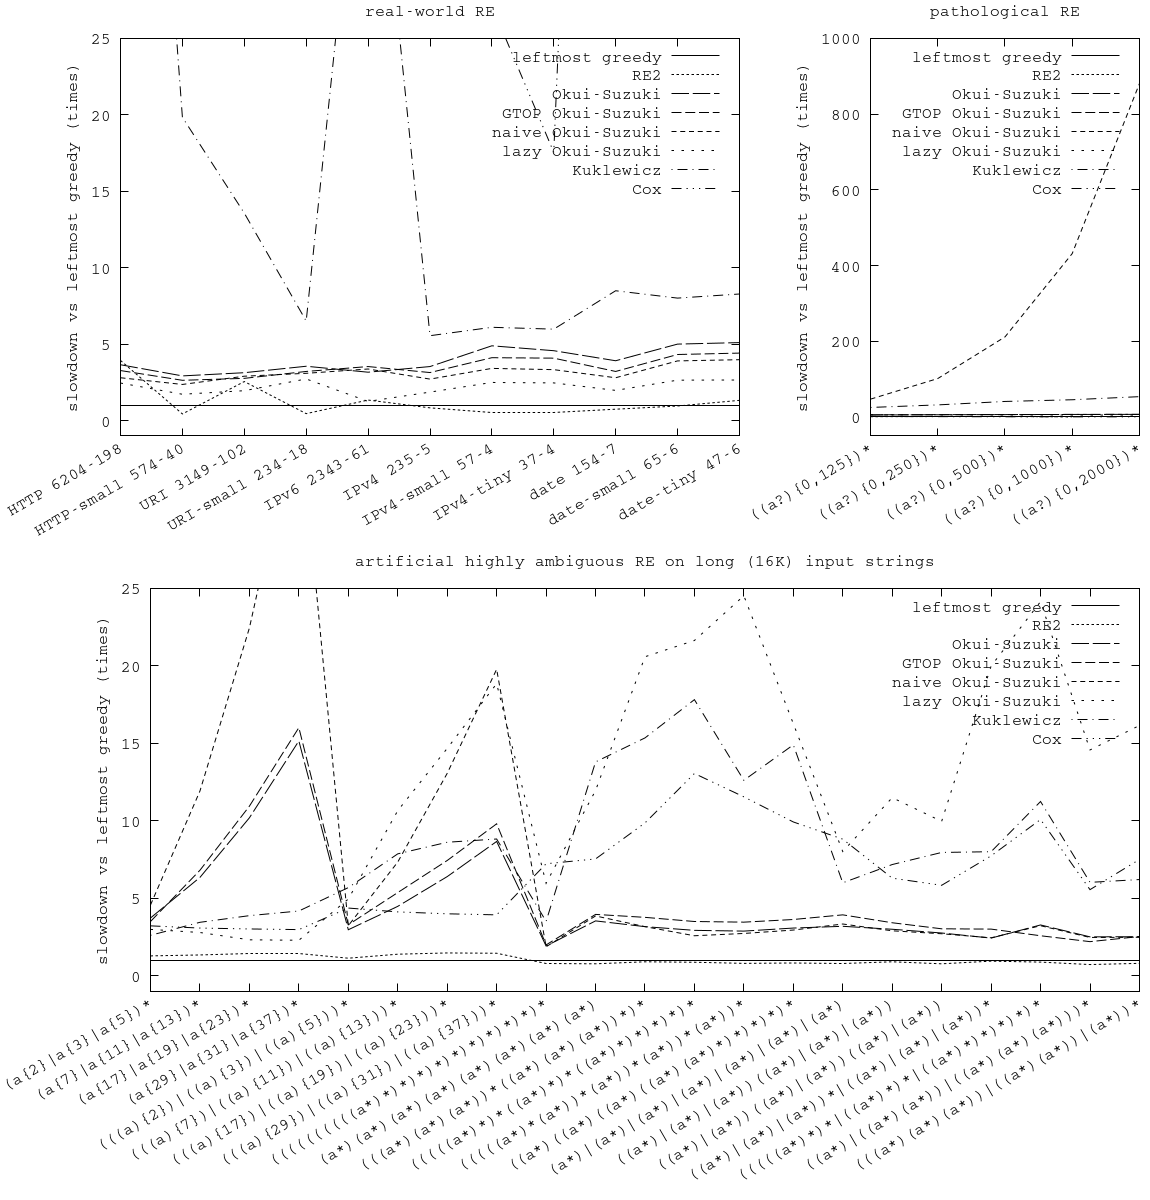
\includegraphics[width=\linewidth]{img/bench/plot.png}
\vspace{-2em}
\caption{
Benchmarks.\\
Real-world tests have labels of the form ``title $m$-$k$'', where $m$ is RE size and $k$ is the number of capturing groups.
%: real-world RE (upper left),
%pathological RE for naive precedence table algorithm (upper right),
%artifical highly ambiguous RE on very long inputs (lower).
}
\end{figure}

\begin{itemize}[itemsep=0.5em]
    \item Okui-Suzuki algorithm degrades with increased closure size.
        This is understandable, as the algorithm performs pairwise comparison of closure states to compute precedence matrices.
        Naive $update \Xund ptables ()$ algorithm degrades extremely fast,
        and the advanced algorithm behaves much better (though it may incur slight overhead in simple cases).

    \item Kuklewicz algorithms degrades with increased closure size and increased number of tags.
        This is not surprizing, as the algorithm has per-state and per-tag loop used to compute precedence matrix.
        On real-world tests with many capturing groups Kuklewicz algorithm is much slower than Okui-Suzuki algorithm.

    \item Cox algorithm degrades with increased number of tags.
        The bottleneck of the algorithm is copying of offset arrays
        (each array contains a pair of offsets per tag).
        Using GOR1 instead of naive depth-first search increases the amount of copying (though asymptotically faster),
        because depth-dirst scan order allows to use a single buffer array that is updated and restored in-place.
        However, copying is required elsewhere in the algorithm,
        and in general it is not suited for RE with many submatch groups.
        On real-world tests Cox algorithm is so slow that it did not fit into the plot space.

    \item Lazy variation of Okui-Suzuki degrades with increased cache size and the size of path context.
        This may happen because of long input strings and because of high level of ambiguity in RE
        (in such cases lazy algorithm does all the work of non-lazy algorithm,
        but with the additional overhead on cache lookups/insertions and accumulation of data from the previous steps).
        On real-world tests lazy variation of Okui-Suzuki is fast.

    \item GOR1 and GTOP performance is similar.

    \item RE2 performance is close to our leftmost greedy implementation.
    \\[-0.5em]
\end{itemize}

One particularly interesting group of tests that show the above points
are RE of the form $(a^{k_1}|\hdots|a^{k_n})^{0,\infty}$
(artificial tests 1-4)
and their variations with more capturing groups
(artificial tests 5-8).
For example, consider \texttt{(a\{2\}|a\{3\}|a\{5\})*} and \texttt{(((a)\{2\})|((a)\{3\})|((a)\{5\}))*}.
Given input string \texttt{a...a},
submatch on the last iteration varies with the length of input:
it equals \texttt{aaaaa} for $5n$-character string,
\texttt{aa} for strings of length $5n - 3$ and $5n - 1$,
and \texttt{aaa} for strings of length $5n - 2$ and $5n + 1$ ($n \in \YN$).
Variation continues infinitely with a period of five characters.
%
We can increase variation period and the range of possible submatch results by choosing larger counter values.
%
This causes increased closure size ---
hence the slowdown of Okui-Suzuki algorithm on tests 1 to 4 and 5 to 8 (especially pronounced for the ``naive Okui-Suzuki'' variation),
and the more gentle slowdown of Kuklewicz algorithm on the same ranges.
%
Adding more capturing groups increases the number of tags ---
hence the slowdown of Kuklewicz and Cox algorithms on 5-8 group compared to 1-4 group.
%
%Note that Cox algorithm performs very well on this test and slows down at the same pace as leftmost greedy.
\\

In closing, we would like to point out that correctness
of all benchmarked implementations has been tested on a subset of Glenn Fowler test suite [??]
(we removed tests for backreferences and start/end anchors),
extended by Kuklewicz and further extended by ourselves to some 500 tests.
All algorithms except Cox algorithm have passed the tests
(Cox algorithm fails in about 10 cases for the reasons discussed in the introduction).

\FloatBarrier


\section{Conclusions and future work}

The main result of our work is a practical POSIX matching algorithm
that can be used on real-world regular expressions,
does not require complex preprocessing
and incurs relatively modest disambiguation overhead compared to other algorithms.
%
We tried to present the algorithm in full, with a few useful variations,
in order to make implementation easy for the reader.
\\

We see a certain tradeoff between speed and memory usage:
bounded-memory version of the algorithm performs a lot of redundant work,
and the lazy version avoids redundant work at the expense of potentially unbounded memory usage.
Both approaches seem not ideal;
perhaps in practice a hybrid approach can be used.
\\

It is still an open question to us
whether it is possible to combine the elegance of derivative-based approach to POSIX disambiguation
with the practical efficiency of NFA-based methods.
%
Derivative-based approach constructs match results in such order that longest-leftmost result is always first.
%
We experimented with recursive descent parsers that embrace the same ordering idea,
but the resulting algorithm was rather complex and slow in practice.
\\

It would be interesting to apply our approach to automata with counters
instead of unrolling bounded repetition.


\vfill\null
\clearpage


\section*{Appendix}

\subsection*{Proof of theorem \ref{theorem_porder_on_PTs}}

\begin{theoremEnd}[normal, no link to proof, no link to theorem]{lemma}
[Unique position mapping from all PTs to IRE]
    \label{lemma_positions}
    If $t, s \in PT(e)$ for some RE $e$
    and there is a common position $p \in Pos(t) \cap Pos(s)$,
    then $p$ corresponds to the same position $p' \in Pos(\IRE(e))$ for both $t$ and $s$.
\end{theoremEnd}
\begin{proofEnd}
    The proof is by induction on the length of $p$.
    Let $r = \IRE(e)$.
    Induction basis: $p = p' = \Lambda$ (the roots of $t$ and $s$ correspond to the root of $e$).
    Induction step: suppose that for any position $p$ of length $|p| < h$ the lemma is true.
    We will show that if exists $k \in \YN$ such that $p.k \in Pos(t) \cap Pos(s)$,
    then $p.k$ corresponds to the same position $p'.k'$ in $r$ for both $t$ and $s$ (for some $k' \in \YN$).
    If $r|_{p'}$ is an elementary IRE of the form $(i, j, \epsilon)$ or $(i, j, \alpha)$,
    or if at least one of $t|_p$ and $s|_p$ is $\varnothing$,
    then $k$ doesn't exist.
    Otherwise $r|_{p'}$ is a compound IRE and both $t|_p$ and $s|_p$ are not $\varnothing$.
    If $r|_{p'}$ is a union $(i, j, (i_1, j_1, r_1)|(i_2, r_2, j_2))$
    or a product $(i, j, (i_1, j_1, r_1)\cdot(i_2, r_2, j_2))$,
    then both $t|_p$ and $s|_p$ have exactly two subtrees,
    and positions $p.1$ and $p.2$ in $t$ and $s$ correspond to positions $p'.1$ and $p'.2$ in $r$.
    Otherwise, $r|_{p'}$ is a repetition $(i, j, r_1^{n,m})$
    and for any $k \geq 1$ position $p.k$ in $t$ and $s$ corresponds to position $p'.1$ in $r$.
\end{proofEnd}

\printProofs[theorem_porder_on_PTs]


\subsection*{Proof of theorem \ref{theorem_sorder_on_PTs}}

\begin{theoremEnd}[normal, no link to proof, no link to theorem]{lemma}
    \label{lemma_incomparability_equivdef}
    If $t, s \in PT(e, w)$ for some RE $e$ and string $w$,
    then $t \sim s \Leftrightarrow \; \forall p : \snorm{t}{p} = \snorm{s}{p}$.
\end{theoremEnd}
\begin{proofEnd}
    Forward implication: let $t \sim s$ and suppose, on the contrary, that $\exists p = min \{ q \mid \snorm{t}{q} \neq \snorm{s}{q} \}$,
    then either $t \prec_p s$ (if $\snorm{t}{p} > \snorm{s}{p}$) or $s \prec_p t$ (if $\snorm{t}{p} < \snorm{s}{p}$),
    both cases contradict $t \sim s$.
    %
    Backward implication: $\forall p : \snorm{t}{p} = \snorm{s}{p}$
    implies $\nexists p : t \prec_p s$ and $\nexists q : s \prec_q t$,
    which implies $t \sim s$.
    \\[0.5em]
\end{proofEnd}

\printProofs[theorem_sorder_on_PTs]


\subsection*{Proof of Theorem \ref{theorem_order_compat}}

\begin{theoremEnd}[normal, no link to proof, no link to theorem]{lemma}
[Comparability of subtrees]
    \label{lemma_subtrees}
    For a giver RE $e$, string $w$ and position $p$,
    if $t, s \in \PT(e, w)$, $p \in Sub(t) \cup Sub(s)$ and $\snorm{t}{q} = \snorm{s}{q} \; \forall q \leq p$,
    then $\exists e', w' : t|_p, s|_p \in \PT(e', w')$.
\end{theoremEnd}
\begin{proofEnd}
    By induction on the length of $p$.
    Induction basis: $p = \Lambda$, let $e' = e$ and $w' = w$.
    %
    Induction step: suppose that the lemma is true for any position $p$ of length
    $|p| < h$, we will show that it is true for any position $p.k$ of length $h$
    ($k \in \YN$).
    %
    Assume that $p.k \in Sub(t) \cap Sub(s)$
    (otherwise either $p.k \not\in Sub(t) \cup Sub(s)$,
    or exactly one of $\snorm{t}{p.k}$, $\snorm{s}{p.k}$ is $\infty$ --- in both
    cases lemma conditions are not satisfied).
    Then both $t|_p$ and $s|_p$ have at least one subtree: let
    $t|_{p} = T(t_1, \dots, t_n)$ and
    $s|_{p} = T(s_1, \dots, s_m)$, where $n, m \geq k$.
    %
    By induction hypothesis $\exists e', w' : t|_p, s|_p \in \PT(e', w')$.
    We have $w' = str(t_1) \dots str(t_n) = str(s_1) \dots str(s_m)$.
    %
    We show that $str(t_k) = str(s_k)$.
    Consider positions $p.j$ for $j \leq k$.
    By defintion the set of submatch positions contains siblings,
    therefore $p.j \in Sub(t) \cap Sub(s)$.
    By lemma conditions $\snorm{t}{p.j} = \snorm{s}{p.j}$ (because $p.j \leq p.k$),
    therefore $|str(t_1) \dots str(t_{k-1})|$
    $= \sum\nolimits_{j=1}^{k-1}\snorm{t}{j}$
    $= \sum\nolimits_{j=1}^{k-1}\snorm{s}{j}$
    $= |str(s_1) \dots str(s_{k-1})|$ and
    $|str(t_k)| = |str(s_k)|$.
    Consequently, $str(t_k)$ and $str(s_k)$ start and end at the same character in $w'$ and therefore are equal.
    %
    Finally, have $t|_{p.k}, s|_{p.k} \in PT(r|_{p.k}, str(t_k))$ and induction step is complete.
\end{proofEnd}

\printProofs[theorem_order_compat]


\subsection*{Proof of Theorem \ref{theorem_order_on_pe_same_as_on_pt}}

%\begin{theoremEnd}[normal, no link to proof, no link to theorem]{lemma}
%    \label{lemma_pe_order_antisymm}
%    The longest-leftmost-precedence relation $<$ is antisymmetric:
%    if $\alpha < \beta$, then $\beta \not< \alpha$.
%\end{theoremEnd}
%\begin{proofEnd}
%    Suppose, on the contrary, that $\alpha < \beta$ and $\beta < \alpha$.
%    Let $\big( (\rho_0, \dots, \rho_n), (\rho'_0, \dots, \rho'_n) \big) = traces(\alpha, \beta)$.
%    %
%    If $\exists i = max \{j \mid \rho_j \neq \rho'_j \}$, then
%    $\alpha < \beta \implies \alpha \sqsubset \beta \implies \rho_i > \rho'_i$, but
%    $\beta < \alpha \implies \beta \sqsubset \alpha \implies \rho'_i > \rho_i$. Contradiction.
%    %
%    Otherwise $\rho_i = \rho'_i \; \forall i$, then
%    $\alpha < \beta \implies \alpha \sim \beta \wedge \alpha \subset \beta$ and
%    $\beta < \alpha \implies \beta \sim \alpha \wedge \beta \subset \alpha$.
%    Let
%    $x = first (\alpha \backslash \beta)$,
%    $y = first (\beta \backslash \alpha)$, then
%    $\alpha \subset \beta \implies x < y$, but
%    $\beta \subset \alpha \implies y < x$. Contradiction.
%\end{proofEnd}

\begin{theoremEnd}[normal, no link to proof, no link to theorem]{lemma}
    \label{lemma_pe_equiv}
    Let $s, t \in PT(e, w)$ for some RE $e$ and string $w$.
    If $s \sim t$, then $\Phi_{h}(s) = \Phi_{h}(t) \; \forall h$.
\end{theoremEnd}
\begin{proofEnd}
    By induction on the height of $e$.
    %
    Induction basis: or height $1$ we have
    $| PT(e, w) | \leq 1 \; \forall w$,
    therefore $s = t$ and $\Phi_{h}(s) = \Phi_{h}(t)$.
    %
    Induction step:
    height is greater than 1, therefore
    $s = T^{d} (s_1, \dots, s_n)$ and
    $t = T^{d} (t_1, \dots, t_m)$.
    If $d = 0$, then $\Phi_{h}(s) = str(s) = w = str(t) = \Phi_{h}(t)$.
    Otherwise $d \neq 0$.
    By lemma \ref{lemma_incomparability_equivdef} we have $s \sim t \Rightarrow \snorm{s}{p} = \snorm{t}{p} \;\forall p$.
    This implies $n = m$ (otherwise the norm of subtree at position $min(n,m)+1$ is $\infty$ for only one of $s$, $t$).
    Therefore
    $\Phi_{h}(s) = \Xl_{h+1} \Phi_{h+1}(s_1), \dots, \Phi_{h+1}(s_n) \Xr_h$ and
    $\Phi_{h}(t) = \Xl_{h+1} \Phi_{h+1}(t_1), \dots, \Phi_{h+1}(t_n) \Xr_h$.
    It suffices to show that $\forall i \leq n: \Phi_{h+1}(s_i) = \Phi_{h+1}(t_i)$.
    We have $\snorm{s_i}{p} = \snorm{t_i}{p} \;\forall p$ (implied by $\snorm{s}{p} = \snorm{t}{p} \;\forall p$),
    therefore by lemma \ref{lemma_incomparability_equivdef} $s_i \sim t_i$,
    and by lemma \ref{lemma_subtrees} $\exists e', w': s_i, t_i \in PT(e', w')$,
    where the height of $e'$ is less than the height of $e$.
    By induction hypothesis $\Phi_{h+1}(s_i) = \Phi_{h+1}(t_i)$.
\end{proofEnd}

\begin{theoremEnd}[normal, no link to proof, no link to theorem]{lemma}
    \label{lemma_pe_less_1}
    Let $s, t \in PT(e, w)$.
    If $s \prec_p t$ and $|p| = 1$, then $\Phi_{h}(s) < \Phi_{h}(t) \; \forall h$.
\end{theoremEnd}
\begin{proofEnd}
    By lemma conditions $|p| = 1$, therefore $p \in \YN$.
    At least one of $s|_p$ and $t|_p$ must exist (otherwise $\snorm{s}{p} = \infty = \snorm{t}{p}$ which contradicts $s \prec_p t$),
    therefore $e$ is a compound RE and $s$, $t$ can be represented as
    $s = T^{d} (s_1, \dots, s_n)$ and
    $t = T^{d} (t_1, \dots, t_m)$
    where $d \neq 0$ because $\Lambda$ is a prefix of decision position $p$.
    Let $k$ be the number of frames and let $j$ be the fork, then:
    \begin{alignat*}{7}
        \Phi_{h}(s) &\;=\; \Xl_{h+1} &&\Phi_{h+1}(s_1) &&\dots &&\Phi_{h+1}(s_n) \Xr_h
            &&\;=\; \beta_0 a_1 \dots a_j \beta_j &&\;\big|\; && \gamma_j a_{j + 1} \dots a_k \gamma_k \\[-0.5em]
        \Phi_{h}(t) &\;=\; \Xl_{h+1} &&\Phi_{h+1}(t_1) &&\dots &&\Phi_{h+1}(t_m) \Xr_h
            &&\;=\; \beta_0 a_1 \dots a_j \beta_j &&\;\big|\; && \delta_j a_{j + 1} \dots a_k \delta_k
    \end{alignat*}
%
    Consider any $i < p$ ($i \in \YN$).
    By lemma conditions $s \prec_p t$, therefore $\snorm{s}{q} = \snorm{t}{q} \;\forall q < p$, and
    in particular $\snorm{s_i}{q} = \snorm{t_i}{q} \;\forall q$, therefore
    by lemma \ref{lemma_incomparability_equivdef} $s_i \sim t_i$,
    therefore by lemma \ref{lemma_pe_equiv} $\Phi_{h+1}(s_i) = \Phi_{h+1}(t_i)$.
    Let $traces (\Phi_{h}(s), \Phi_{h}(t)) = \big( (\rho_0, \dots, \rho_k), (\rho'_0, \dots, \rho'_k) \big)$.

    \begin{itemize}[itemsep=0.5em, topsep=0.5em]
    \item[(1)]
        Case $\infty = \snorm{s}{p} > \snorm{t}{p}$.
        In this case $s_p$ does not exist
        and fork happens immediately after $\Phi_{h+1}(s_{p-1})$, $\Phi_{h+1}(t_{p-1})$:
        \begin{alignat*}{7}
            \Phi_{h}(s) &\;=\; \Xl_{h+1} &&\Phi_{h+1}(s_1) &&\dots &&\Phi_{h+1}(s_{p-1})
                &&\;\big|\; \Xr_{h}         &&      && \\[-0.5em]
            \Phi_{h}(t) &\;=\; \Xl_{h+1} &&\Phi_{h+1}(t_1) &&\dots &&\Phi_{h+1}(t_{p-1})
                &&\;\big|\; \Phi_{h+1}(t_p) &&\dots &&\Phi_{h+1}(t_m) \Xr_{h}
        \end{alignat*}
        %
        Fork frame is the last one,
        therefore both $\gamma_j$ and $\delta_j$ contain the closing parenthesis $\Xr_{h}$
        and we have $\rho_j = \rho'_j = h$.
        For all $i < j$ we have $\rho_i = \rho'_i = -1$.
        Therefore $\rho_i = \rho'_i \;\forall i$ and $\Phi_{h}(s) \sim \Phi_{h}(t)$.
        Since $first(\gamma_j)$ is $\Xr$ and $first(\delta_j)$ is one of $\Xl$ and $\Xm$,
        we have $\Phi_{h}(s) \subset \Phi_{h}(t)$.
        Therefore $\Phi_{h}(s) < \Phi_{h}(t)$.

    \item[(2)]
        Case $\infty > \snorm{s}{p} > \snorm{t}{p} = -1$.
        In this case both $s_p$ and $t_p$ exist,
        $s_p$ is not $\varnothing$ and $t_p$ is $\varnothing$,
        and fork happens immediately after $\Phi_{h+1}(s_{p-1})$, $\Phi_{h+1}(t_{p-1})$:
        \begin{alignat*}{8}
            \Phi_{h}(s) &\;=\; \Xl_{h+1} &&\Phi_{h+1}(s_1) &&\dots &&\Phi_{h+1}(s_{p-1})
                &&\;\big|\; \Xl_{h+2} \; x \; \Xr_{h+1} \; &&\Phi_{h+1}(s_{p+1}) &&\dots &&\Phi_{h+1}(s_n) \Xr_{h} \\[-0.5em]
            \Phi_{h}(t) &\;=\; \Xl_{h+1} &&\Phi_{h+1}(t_1) &&\dots &&\Phi_{h+1}(t_{p-1})
                &&\;\big|\; \Xm_{h+1} \;\;\;\;\;\;         &&\Phi_{h+1}(t_{p+1}) &&\dots &&\Phi_{h+1}(t_m) \Xr_{h}
        \end{alignat*}
        %
        \begin{itemize}
        \item[(2.1)]
            If fork frame is the last one,
            then both $\gamma_j$ and $\delta_j$ contain the closing parenthesis $\Xr_{h}$
            and we have $\rho_j = \rho'_j = h$.

        \item[(2.2)]
            Otherwise fork frame is not the last one.
            We have $minh(\gamma_j)$, $minh(\delta_j) \geq h + 1$
            and $lasth (\beta_j) = h + 1$
            (the last parenthesis in $\beta_j$ is either $\Xl_{h+1}$ if $p = 1$ and $s_{p-1}$ does not exist,
            or else one of $\Xr_{h+1}$ and $\Xm_{h+1}$),
            therefore $\rho_j = \rho'_j = h + 1$.
            %
            For subsequent frames $i$ such that $j < i < k$ we have $\rho_i = \rho'_i = h + 1$
            (on one hand $\rho_i, \rho'_i \leq h + 1$ because $\rho_j = \rho'_j = h + 1$,
            but on the other hand $minh(\gamma_i)$, $minh(\delta_i) \geq h + 1$).
            %
            For the last pair of frames we have $\rho_k = \rho'_k = h$ (they both contain the closing parenthesis $\Xr_{h}$).
        \end{itemize}

        In both cases $\rho_i = \rho'_i \;\forall i \geq j$.
        Since $\rho_i = \rho'_i = -1 \;\forall i < j$,
        we have $\rho_i = \rho'_i \;\forall i$ and therefore $\Phi_{h}(s) \sim \Phi_{h}(t)$.
        %
        Since $first (\gamma_j) = \Xl < \Xm = first (\delta_j)$ we have $\Phi_{h}(s) \subset \Phi_{h}(t)$.
        Therefore $\Phi_{h}(s) < \Phi_{h}(t)$.

    \item[(3)]
        Case $\infty > \snorm{s}{p} > \snorm{t}{p} \geq 0$.
        In this case both $s_p$ and $t_p$ exist and none of them is $\varnothing$,
        and fork happens somewhere after the opening parenthesis $\Xl_{h+2}$
        and before the closing parenthesis $\Xr_{h+1}$ in $\Phi_{h}(s_p)$, $\Phi_{h}(t_p)$:
        \begin{alignat*}{9}
            \Phi_{h}(s) &\;=\; \Xl_{h+1} &&\Phi_{h+1}(s_1) &&\dots &&\Phi_{h+1}(s_{p-1}) &&\; \Xl_{h+2} \; x
                &&\;\big|\; y \; \Xr_{h+1} \; &&\Phi_{h+1}(s_{p+1}) &&\dots &&\Phi_{h+1}(s_n) \Xr_{h} \\[-0.5em]
            \Phi_{h}(t) &\;=\; \Xl_{h+1} &&\Phi_{h+1}(t_1) &&\dots &&\Phi_{h+1}(t_{p-1}) &&\; \Xl_{h+2} \; x
                &&\;\big|\; z \; \Xr_{h+1} \; &&\Phi_{h+1}(t_{p+1}) &&\dots &&\Phi_{h+1}(t_m) \Xr_{h}
        \end{alignat*}
        %
        From $\snorm{s}{p} > \snorm{t}{p} \geq 0$ it follows that
        $s_p$ contains more alphabet symbols than $t_p$.
        Consequently $\Phi_{h+1}(s_p)$ contains more alphabet symbols, and thus spans more frames than $\Phi_{h+1}(t_p)$.
        %
        Let $l$ be the index of the frame $\delta_l$ that contains the closing parenthesis $\Xr_{h+1}$ of $\Phi_{h+1}(t_p)$.
        By the above reasoning $\Phi_{h+1}(s_p)$ does not end in frame $\gamma_l$,
        therefore $\gamma_l$ does not contain the closing parenthesis $\Xr_{h+1}$
        and we have $minh (\gamma_l) \geq h+2$ and $minh (\delta_l) = h+1$.
        %
        Furthermore, note that $minh(x)$, $minh(y)$, $minh(z) \geq h + 2$,
        therefore $lasth(\beta_j) \geq h+2$ (including the case when $x$ is empty),
        and for all frames $i$ such that $j \leq i < l$ (if any) we have $\rho_i, \rho'_i \geq h+2$.
        %
        Consequently, for $l$-th frame we have $\rho_l \geq h+2$ and $\rho'_l = h + 1$, thus $\rho_l > \rho'_l$.
        %
        For subsequent frames $i$ such that $l < i < k$ we have $minh(\gamma_i)$, $minh(\delta_i) \geq h + 1$,
        therefore $\rho_i \geq h+1$ and $\rho'_i = h + 1$, thus $\rho_i \geq \rho'_i$.
        %
        For the last pair of frames we have $\rho_k = \rho'_k = h$, as they both contain the closing parenthesis $\Xr_{h}$.
        %
        Therefore $\Phi_{h}(s) \sqsubset \Phi_{h}(t)$,
        which implies $\Phi_{h}(s) < \Phi_{h}(t)$.
    \end{itemize}
\end{proofEnd}

\begin{theoremEnd}[normal, no link to proof, no link to theorem]{lemma}
    \label{lemma_pe_less}
    Let $s, t \in PT(r, w)$.
    If $s \prec_p t$, then $\Phi_{h}(s) < \Phi_{h}(t) \; \forall h$.
\end{theoremEnd}
\begin{proofEnd}
    The proof is by induction on the length of $p$.
    %
    Induction basis for $|p| = 1$ is given by lemma \ref{lemma_pe_less_1}.
    %
    Induction step: suppose that the lemma is correct for all $p$ of length $|p| < h$ and let $|p| = h$ ($h \geq 2$).
    %
    Let $p = p'.p''$ where $p' \in \YN$.
    %
    At least one of $s|_p$ and $t|_p$ must exist (otherwise $\snorm{s}{p} = \infty = \snorm{t}{p}$ which contradicts $s \prec_p t$),
    therefore both $e$ and $e|_{p'}$ are compound RE and $s$, $t$ can be represented as
    $s = T^{d} (s_1, \dots, s_n)$ and
    $t = T^{d} (t_1, \dots, t_m)$ where
    $s' = s_{p'} = T^{d'} (s'_1, \dots, s'_{n'})$ and
    $t' = t_{p'} = T^{d'} (t'_1, \dots, t'_{m'})$
    and both $d, d' \neq 0$ (because $\Lambda$ and $p'$ are prefixes of decision position $p$).
    %
    Therefore $\Phi_{h}(s)$, $\Phi_{h}(t)$ can be represented as follows:
    \begin{alignat*}{9}
        \Phi_{h}(s)
            \;&=
                \;&& \Xl_{h+1} \Phi_{h+1}(s_1) \dots \Phi_{h+1}(s_{p'-1})
                \;&& \overbrace {\Xl_{h+2} \Phi_{h+2}(s'_1) \dots \Phi_{h+2}(s'_{n'}) \Xr_{h+1}}^{\Phi_{h+1}(s')}
                \;&& \Phi_{h+1}(s_{p'+1}) \Phi_{h+1}(s_n) \Xr_{h}
                \\
        \Phi_{h}(t)
            \;&=
                \;&& \Xl_{h+1} \Phi_{h+1}(t_1) \dots \Phi_{h+1}(t_{p'-1})
                \;&& \underbrace {\Xl_{h+2} \Phi_{h+2}(t'_1) \dots \Phi_{h+2}(t'_{m'}) \Xr_{h+1}}_{\Phi_{h+1}(t')}
                \;&& \Phi_{h+1}(t_{p'+1}) \Phi_{h+1}(t_m) \Xr_{h}
    \end{alignat*}
    %
    Consider any $i < p'$.
    By lemma conditions $s \prec_p t$, therefore $\snorm{s}{q} = \snorm{t}{q} \;\forall q < p$, and
    in particular $\snorm{s_i}{q} = \snorm{t_i}{q} \;\forall q$, therefore
    by lemma \ref{lemma_incomparability_equivdef} $s_i \sim t_i$,
    therefore by lemma \ref{lemma_pe_equiv} $\Phi_{h+1}(s_i) = \Phi_{h+1}(t_i)$.
    %
    Since $p' < p$ we have $\snorm{s}{q} = \snorm{t}{q} \;\forall q \leq p'$ and
    by lemma \ref{lemma_subtrees} $\exists e', w' : s', t' \in PT(e', w')$.
    Since $\snorm{s'}{q} = \snorm{s}{p'.q} \;\forall q$
    and $\snorm{t'}{q} = \snorm{t}{p'.q} \;\forall q$,
    we have $s' \prec_{p''} t'$.
    Since $|p''| < |p|$ by induction hypothesis we have $\Phi_{h+1}(s') < \Phi_{h+1}(t')$.
    %
    If $j$ is the fork and $f \leq j \leq k$, then
    $\Phi_{h}(s)$, $\Phi_{h}(t)$ can be represented as:
    \begin{alignat*}{9}
        \Phi_{h}(s)
            \;&=
                \;&& \beta_0 a_1 \dots a_f \beta_f^1
                \;&& \overbrace {\beta_f^2  a_{f+1} \dots a_j \beta_j \;\big|\; \gamma_j a_{j+1} \dots a_k \gamma_k^1}^{\Phi_{h+1}(s')}
                \;&& \gamma_k^2 a_{k+1} \dots a_l \gamma_l
                \\[-0.5em]
        \Phi_{h}(t)
            \;&=
                \;&& \beta_0 a_1 \dots a_f \beta_f^1
                \;&& \underbrace {\beta_f^2  a_{f+1} \dots a_j \beta_j \;\big|\; \delta_j a_{j+1} \dots a_k \delta_k^1}_{\Phi_{h+1}(t')}
                \;&& \delta_k^2 a_{k+1} \dots a_l \delta_l
    \end{alignat*}
    %
    Let $traces (\Phi_{h}(s), \Phi_{h}(t)) = \big( (\rho_0, \dots, \rho_l), (\rho'_0, \dots, \rho'_l) \big)$
    and $traces (\Phi_{h+1}(s'), \Phi_{h+1}(t')) = \big( (\sigma_h, \dots, \sigma_k), (\sigma'_h, \dots, \sigma'_k) \big)$.
    %
    We show that for frames $i$ such that $j \leq i < k$ we have
    $\rho_i = \sigma_i \wedge \rho'_i = \sigma'_i$
    and for subsequent frames $k \leq i \leq l$ we have $\rho_i = \rho'_i$.
    %
    \begin{itemize}[itemsep=0.5em, topsep=0.5em]
    \item[(1)]
        Case $i = j < k \leq l$ (the fork frame).
        Since we have shown that $\Phi_{h+1}(s_i) = \Phi_{h+1}(t_i) \;\forall i < p'$,
        and since $\Phi_{h+1}(s')$ and $\Phi_{h+1}(t')$ have nonempty common prefix $\Xl_{h+2}$,
        it follows that $lasht (\Phi_{h}(s) \sqcap \Phi_{h}(t)) = lasth (\Phi_{h+1}(s') \sqcap \Phi_{h+1}(t'))$.
        %
        From $j < k$ it follows that $\gamma_j$ and $\delta_j$ end before $a_k$
        and are not changed by appending $\gamma^2_k$ and $\delta^2_k$.
        %
        Therefore $\rho_j = \sigma_j \wedge \rho'_j = \sigma'_j$.

    \item[(2)]
        Case $j < i < k \leq l$.
        The computation of $\rho_i$, $\rho'_i$ depends only on
        $\rho_j$, $\rho'_j$,
        or which we have shown $\rho_j = \sigma_j \wedge \rho'_j = \sigma'_j$ in case (1),
        and on $\Phi_{h+1}(s')$, $\Phi_{h+1}(t')$,
        which are not changed by appending $\gamma^2_k$ and $\delta^2_k$ since $i < k$.
        Therefore $\rho_i = \sigma_i \wedge \rho'_i = \sigma'_i$.

    \item[(3)]
        Case $j \leq i = k < l$. We have
        $minh (\gamma^1_k) = minh (\delta^1_k) = h + 1$ and
        $minh (\gamma^2_k) = minh (\delta^2_k) \geq h + 1$.
        None of the preceding frames after the fork contain parentheses with height less than $h + 1$,
        therefore $\rho_k = \rho'_k = h + 1$.

    \item[(4)]
        Case $j \leq k < i < l$.
        We have $\rho_i = \rho'_i = h + 1$,
        because $\rho_k = \rho'_k = h + 1$ and $minh(\gamma_i)$, $minh(\delta_i) \geq h + 1$.

    \item[(5)]
        Case $j \leq k \leq i = l$.
        We have $\rho_l = \rho'_l = h$,
        because both $\gamma_l$ and $\delta_l$ contain the closing parenthesis $\Xr_{h}$.
    \end{itemize}
    %
    We have shown that $\rho_i = \sigma_i \wedge \rho'_i = \sigma'_i \;\forall i: j \leq i < k$
    and $\rho_i = \rho'_i \;\forall i: k \leq i \leq l$.
    It trivially follows that $\Phi_{h+1}(s') \sqsubset \Phi_{h+1}(t')$ $\Rightarrow \Phi_{h}(s) \sqsubset \Phi_{h}(t)$
    and $\Phi_{h+1}(s') \sim \Phi_{h+1}(t')$ $\Rightarrow \Phi_{h}(s) \sim \Phi_{h}(t)$.
    Because none of $\Phi_{h+1}(s')$, $\Phi_{h+1}(t')$ is a proper prefix of another,
    $\Phi_{h+1}(s') \subset \Phi_{h+1}(t')$ $\Rightarrow \Phi_{h}(s) \subset \Phi_{h}(t)$.
    Therefore $\Phi_{h+1}(s') < \Phi_{h+1}(t') \Rightarrow \Phi_{h}(s) < \Phi_{h}(t)$
    (the premise has been shown).
\end{proofEnd}

\printProofs[theorem_order_on_pe_same_as_on_pt]


\subsection*{Correctness of incremental path comparison}

\printProofs[lemma_frames]
\printProofs[lemmata_closure]

\iffalse
\begin{figure}\label{fig_gor1}
\includegraphics[width=\linewidth]{img/gor1.pdf}
\caption{Sub-TNFA for individual sub-RT with submatch groups: \\
(a) -- union, (b) -- product, (c), (d) -- bounded repetition, (e), (f) -- unbounded repetition.}
\end{figure}
\fi


\end{document}

